\documentclass{hhuthesis}

\usepackage[english,ngerman]{babel} % Deutsch

\author{Tom Schreiner}
\title{Visualisieren von Algorithmen in Compilern}
\gratuationtype{Bachelor}

%% Beginn- und Abgabedaten der Arbeit
\begindate{05. November 2024} % Beginn
\duedate{05. Februar 2025} % Abgabe

%% Erst- und Zweitgutachter
\firstexaminer{John~Witulski}
\secondexaminer{Fabian~Ruhland}

\usepackage[textsize=scriptsize]{todonotes}

%% Zeige Zeilennummern in der Arbeit an.
%% Der \linenumbers Befehl muss hierzu aufgerufen werden.
%% Praktisch für Feedback Ihrer potentiellen Korrekturleser!
\usepackage{lineno}
% \linenumbers % <- Kommentar entfernen!


%% Häufig benutzte mathematische Packages.
\usepackage{amsfonts}
\usepackage{amsmath}
\usepackage{amssymb}

\usepackage{wrapfig}
\usepackage{listings} % Einbindung von Code
\usepackage{algorithmicx} % Angabe von Algorithmen in Pseudocode
\usepackage{siunitx} % \num Befehl zum einfacheren Formatieren von Zahlen.
\usepackage{enumitem} % Leichter konfigurierbare enumerate-Umgebungen.
\usepackage{subcaption} % Unterteilung von Figures in Subfigures.
\usepackage{hyperref} % Klickbare Referenzen (z.B. im Inhaltsverzeichnis)
\usepackage{url} % \url Kommando für Darstellung von Links
\usepackage{csquotes} % Improved quoting.
\usepackage{xspace} % Nicht terminierte Kommandos essen keinen Whitespace mehr.

%% Tabellen
\usepackage{tabularx} % tabularx Umgebung für mehr Kontrolle über Tabellen.
\usepackage{booktabs} % \toprule, \midrule, \bottomrule
\usepackage{multirow}
\usepackage{multicol}
\usepackage{longtable} % Große Tabellen gehen über mehrere Seiten.

%% Intelligenteres Referenzieren mittels \cref.
%% \languagename um dynamisch zwischen ngerman oder english zu wechseln.
\usepackage[\languagename,capitalize]{cleveref}

%%%%%%%%%%%%%%%%%%%%%%%%%%%%%%%%%%%%%%%%%%%%%%%%%%%%%%%%%%%%%%%%%%%%%%%%%%%%%%%%
%% (Ende) LaTeX Packages in Nutzung                                           %%
%%%%%%%%%%%%%%%%%%%%%%%%%%%%%%%%%%%%%%%%%%%%%%%%%%%%%%%%%%%%%%%%%%%%%%%%%%%%%%%%


\begin{document}
%% Set up title page, declaration of authorship, abstract, acknowledgements
\frontmatter
\makefrontmatter
\tableofcontents

\mainmatter

%%%%%%%%%%%%%%%%%%%%%%%%%%%%%%%%%%%%%%%%%%%%%%%%%%%%%%%%%%%%%%%%%%%%%%%%%%%%%%%%
%% Der Inhalt der Arbeit                                                      %%
%%                                                                            %%
%% Hier können Sie die schriftliche Ausarbeitung ihrer Arbeit                 %%
%% niederschreiben. Der Übersicht halber bietet sich jedoch an, dies in einer %%
%% oder mehreren separaten Dateien zu tun, welche mittels \input eingebunden  %%
%% werden --- wie auch in der Vorlage geschieht.                              %%
%%%%%%%%%%%%%%%%%%%%%%%%%%%%%%%%%%%%%%%%%%%%%%%%%%%%%%%%%%%%%%%%%%%%%%%%%%%%%%%%

%!TeX root: thesis.tex
\section{Einleitung}
\subsection{Motivation} \label{motiv}
Als ich im Wintersemester das Modul "Compilerbau"\ 
belegt habe, habe ich mich das erste Mal mit
einigen Algorithmen beschäftigt, die eben in diesem
Themengebiet angewendet werden. Dabei fiel es mir
bei einigen schwer, mir diese ohne weiteres
vorzustellen. Ein Tool, mit dem man Schritt für Schritt 
durch diese Algorithmen gehen kann, hätte mir das Verstehen der Algorithmen
und vor allem das Entwickeln einer Intuition, warum diese Algorithmen überhaupt
so funktionieren wie sie es tun stark erleichtert.\\

Es gibt zwar solche Tools, zum Beispiel VisOpt\cite{VisOpt} oder DFAV\cite{dfav},
diese benutzen allerdings ein Subset von Java und JavaScript.
Da im Modul \glqq Compilerbau\grqq sämtliche Algorithmen auf drei Address Code
erklärt werden, passen diese Tools nicht in den Usecase der Studenten.\\

In dieser Bachelorarbeit wird ein Framework in Java
entwickelt, mit dem es einfach sein soll,
Algorithmen zu visualisieren.\\

Im Jahr 2016 wurde von Fabian Ruhland und Isabel Wingen bereits ein ähnliches
Framework entwickelt \cite{toolbox}. Dieses ist leider mittlerweile nicht mehr
mit aktuellen Java-Versionen kompatibel, daher wurde sich dazu entschieden,
ein komplett neues Framework zu entwickeln.\\

Zudem werden einige der Algorithmen, die im Compilerbau verwendet werden,
implementiert. Das Framework basiert darauf, dass durch
Implementierung von Interfaces einfach neue Algorithmen 
als Plugins hinzugefügt werden können. Dadurch kann gewährleistet werden,
dass wenn etwas im Framework nicht mehr funktioniert, 
zum Beispiel durch neue Versionen von Java oder einem Update einer Dependency, 
dieses Modul ausgetauscht werden kann, ohne die implementierten Plugins 
aktualisieren zu müssen.


\newpage
\subsection{Theoretische Grundlagen}
Im folgenden Abschnitt werden die für diese Arbeit notwendigen 
grundlegenden Konzepte und Algorithmen erklärt, da im weiteren 
Verlauf der Arbeit nur auf die Implementierung dieser eingegangen wird.


\subsubsection{Drei Adress Code} \label{t:tac}
Drei Adress Code ist eine Art von Zwischencode
\footnote{Zwischencode hat viele Nutzungsgebiete in einem Compiler,
einerseits verbindet er das Frontend (welches den Quellcode einließt) mit dem
Backend (welches den Maschinencode ausgibt), andererseits ist Zwischencode 
plattformunabhängig, sodass maschinenunabhängige Optimierungen und Analysen auf
diesem ausgeführt werden können.}. 
Charakterisierend für Drei Adress Code (folgend auch 3-Address-Code genannt)
ist, dass einzelne Instruktionen auf maximal drei Adressen (oder Konstanten) 
zugreifen. Die Addresse in die der resultierende Wert gespeichert wird und 
eine oder zwei Addressen oder Konstanten aus denen sich der resultierende Wert bildet.
Dazu ist noch die Operation, die ausgeführt wird angegeben.\\

Für diese Bachelorarbeit wurde eine Teilmenge des im Drachenbuch \cite[Kapitel 6.2.1]{D}
beschriebenen 3-Address-Code verwendet.\\
Folgende Operationen gibt es:
\begin{enumerate}
  \item Binäre Operationen X = Y op Z\\
    in denen das Resultat aus einer der folgenden binären Operation
    in der Adresse X gespeichert wird. Implementiert wurden Addition, 
    Subtraktion, Multiplikation und Division.
  \item Die unäre Operation X = - Y\\
    in der der invertierte Wert von Y in X gespeichert wird.
  \item Der Kopierbefehl X = Y\\
    in der der Wert, der in Adresse Y gespeichert ist, in X kopiert wird.
  \item Der unbedingte Sprung goto X\\
    hier wird kein Wert gespeichert, sondern zu der Adresse die in X gespeichert ist gesprungen
  \item Die bedingten Sprünge if Y goto X und ifFalse Y goto X\\
    mit denen, wenn der Wert Y entweder $wahr$ oder $falsch$ repräsentiert 
    zur Adresse X gesprungen wird  
    oder die nächste Instruktion ausgeführt wird, wenn dies nicht der Fall ist.
  \item Die bedingten Sprünge if Y relOp Z goto X\\
    in denen auch zu X gesprungen wird, wenn die Relation Y relOp Z $wahr$ ist, 
    sonst wird auch hier die nächste Instruktion ausgeführt.\\
    Die Implementierten Relationen sind: 
    \begin{itemize}
      \item Y $<$ Z
      \item Y $\leq$ Z
      \item Y $>$ Z
      \item Y $\geq$ 
      \item Y $=$ Z
      \item Y $\neq$ Z
    \end{itemize}
\end{enumerate}

Hierbei können die Adressen X, Y und Z beliebige Zeichenfolgen sein, 
Y und Z können außerdem Konstanten sein.
Die einzelnen Elemente jeder Instruktion sind durch ein Leerzeichen von einander
getrennt. Verschiedene Instruktionen werden durch einen Zeilenumbruch getrennt.
Da sich die Algorithmen in dieser Arbeit nicht mit komplexeren Aufgaben wie
Speichermanagement beschäftigen, wurde sich dagegen entschieden, den 3AC
umfangreicher zu modellieren.\\

Ein Beispiel für gültigen 3-Address-Code wäre also:
\begin{lstlisting}[caption={3-Address-Code, der die 5-te Fibonacci Zahl ausrechnet und in x speichert}]
  0: n = 5
  1: fib = 1  
  2: lst = 1
  3: n = n - 2
  4: if n <= 0 goto 10
  5: hlp = lst 
  6: lst = fib
  7: fib = lst + hlp
  8: n = n - 1
  9: goto 4
 10: x = fib
\end{lstlisting}


\subsubsection{Grundblöcke} \label{t:bb}
Grundblöcke sind Instruktionsfolgen eines Zwischencodeprogramms,
die immer zusammen ausgeführt werden \cite[S.619]{D}.
Dies ermöglicht es, einen Block an Instruktionen anzuschauen 
und bestimmte Optimierungsalgorithmen auf sie anzuwenden, 
ohne Gefahr zu laufen, die Semantik des Programmes zu verändern.

\newpage
Um ein Programm in Grundblöcke aufzuteilen, kann man wie folgt vorgehen \cite[S.643]{D}:
\begin{enumerate}
  \item Markiere die erste Instruktion des Programmes als Leader, da diese immer ausgeführt wird.
  \item Markiere alle Instruktionen als Leader, die Ziel eines Sprungs sind oder auf einen Sprung folgen.
  \item Alle Instruktionen, die auf eine markierte Instruktion folgen
    bis zu einer neuen markierten Instruktion, gelten nun als ein Grundblock.
\end{enumerate}

Folgend kann man für jeden Grundblock bestimmen, welche Grundblöcke auf ihn folgen, 
daraus lässt sich ein Flussgraph bestimmen, den wir, da er den Kontrollfluss beschreibt,
folglich Kontrollflussgraphen nennen werden. In diesem stellt jeder Grundblock einen Knoten dar
und jede Kante einen Sprung von einem Grundblock zum anderen.\\

Aus unserem Beispielcode aus dem letzten Kapitel können wir also folgende Instruktionen markieren:
\begin{lstlisting}[caption=Fibonacci 3-Address-Code mit markierten Leadern]
  0: n = 5 //Leader, da erste Instruktion
  1: fib = 1  
  2: lst = 1
  3: n = n - 2
  4: if n <= 0 goto 10 //Leader, da 9 hierhin springt
  5: hlp = lst //Leader, da 4 ein bedingter Sprung ist
  6: lst = fib
  7: fib = lst + hlp
  8: n = n - 1
  9: goto 4
 10: x = fib //Leader, da 9 ein Sprung ist und 4 hierhin springen kann
\end{lstlisting}

Daraus folgt, dass wir folgende Grundblöcke haben:
\begin{enumerate}
  \item Ein Grundblock $B_0$, der die Addressen 0 bis 3 besitzt,
  \item der Block $B_1$, der nur die Addresse 4 hat,
  \item Grundblock $B_2$, der die Addressen 5 bis 9 besitzt
  \item und Block $B_3$, der nur die Addresse 10 besitzt.
\end{enumerate}




\newpage
\subsubsection{Kontrollflussgraphen}
Kontrollflussgraphen sind gerichtete Graphen, deren Knoten aus Grundblöcken und 
deren Kanten aus den jeweilig folgenden Grundblöcken besteht.\\

Um unser Beispiel weiterzuführen, bildet sich folgender Kontrollflussgraph:
\begin{figure}[h]
  \centering
  \begin{tikzpicture}[node distance={15mm}, 0/.style = {draw, circle}]
    \node[0] (0) {$B_0$};
    \node[0] (1) [below of=0] {$B_1$};
    \node[0] (2) [below left of=1] {$B_2$};
    \node[0] (3) [below right of=1] {$B_3$};
    \draw[->] (0) to [out=270, in=90] (1);
    \draw[->] (1) to [out=180, in=90] (2);
    \draw[->] (1) to [out=0, in=90] (3);
    \draw[->] (2) to [out=0, in=270] (1);
  \end{tikzpicture}
  \caption{Resultierender Kontrollflussgraph}
  \label{fig:fib-cfg}
\end{figure}

Auf Kontrollflussgraphen lassen sich nun sogenannte Datenflusswerte definieren.
Diese sind Abstraktionen für die Menge aller möglichen Zustände des Programmes
zu einem bestimmten Zeitpunkt. In Bezug zu einem Kontrollflussgraphen ist dieser
Zeitpunkt immer entweder (direkt) vor der Ausführung des Grundblockes, die $in[B]$ Menge
oder nach der Ausführung dessen, die $out[b]$ Menge.
Je nach dem, was wir analysieren beziehungsweise abstrahieren wollen, ändern sich
die Datenflusswerte, da nur die für die jeweilige Analyse relevanten Informationen
betrachtet werden. Ausserdem abhängig von der spezifischen Analyse ist die
Flussrichtung der Datenflusswerte. Wenn der Datenfluss vorwärts gerichtet ist,
verändert sich die $out[B]$ Menge durch Anwendung einer sogenannten Transferfunktion
auf der $in[B]$ Menge, also gilt:
\[out[B]=f_B(in[B])\] 
\[in[B]=\bigcup_{v\in V_B}out[v]\]
Analog gilt, wenn der Datenfluss
rückwärtsgerichtet ist: 
\[in[B]=f_b(out[B])\]
\[out[B]=\bigcup_{n\in N_B}in[n]\]
Hierbei sind $V_B$ und $N_B$ die Mengen der Vorgänger und Nachfolger
eines Grundblocks $B$.\cite[S.732-734]{D}



\newpage
\subsubsection{Erreichende Definitionen} \label{t:rd}
Dies ist eine der gebräuchlichsten und nützlichsten Datenflussanalysen \cite[S.734]{D}.\\
Mit ihnen können wir herausfinden, welchen Variablen zu einem bestimmten
Zeitpunkt ein Wert zugewiesen ist. Eine Anwendung wäre zum Beispiel zu
kontrollieren, ob eine Variable zu einem bestimmten Zeitpunkt  überhaupt
einen Wert hat \cite[S.734]{D}, sofern die ursprüngliche Programmiersprache dies als 
notwendig erachtet. Man kann aber auch schauen, 
ob die Variable eine Konstante ist und somit Instruktionen gespart werden können.

Für die Berechnung der erreichenden Definitionen bestimmen 
wir folgende Datenflusswerte für jeden Grundblock:
\begin{itemize}
  \item Die $gen_B$ Menge\\
    beschreibt die Adressen aller Instruktionen in einem Grundblock $B$ welche einer Variable einen Wert zuweisen,
    also einen Wert \textit{generieren}. Wenn einer Variable ein Wert mehrmals zugewiesen wurde 
    liegt nur die letzte Zuweisung dieser in der $gen_B$ Menge.
  \item Und die $kill_B$ Menge\\
    beschreibt die Adressen aller Instruktionen welche einer Addresse einen Wert zuweisen, 
    der durch eine Instruktion in der $gen_B$ Menge überschrieben wird.
\end{itemize}

Nun können wir uns herleiten, dass alle Variablen, die in einem Grundblock $B$
definiert werden, ihn auch verlassen, also Teil der $out[B]$ Menge sind.
Zudem verlassen auch alle Definitionen den Grundblock, wenn sie nicht überschrieben wurden.
Demnach ist der Datenfluss vorwärtsgerichtet und es gilt die Transferfunktion:
\[out[B]=gen_B \cup (in[B] \backslash kill_B)\]
Hierbei handelt es sich um einen Fixpunktalgorithmus. Das heißt, wir beginnen
mit $out[B]=\emptyset$ für alle Grundblöcke und iterieren dann so lange über diese,
bis sich keine Menge mehr verändert.\cite[S.739-740]{D}

Für unser Beispiel ergibt sich dann \cref{tab:fib-rd}:

\newpage
\begin{table}[h]
  \centering
  \begin{tabular}{|l|c|c|c|c|}
    \hline
    $B       $&$B_0      $&$B_1          $&$B_2          $&$B_3            $\\\hline
    $gen_B   $&$1,2,3    $&$             $&$5,6,7,8      $&$10             $\\\hline
    $kill_B  $&$0,6,7,8  $&$             $&$1,2          $&$               $\\\hline
    $ in_1[B]$&$         $&$             $&$             $&$               $\\\hline
    $out_1[B]$&$\textcolor{hhudarkblue}{n,fib,lst}$&$$&$\textcolor{hhudarkblue}{n,fib,lst,hlp}$&$\textcolor{hhudarkblue}{x}$\\\hline
    $ in_2[B]$&$         $&$\textcolor{hhudarkblue}{n,fib,lst,hlp}$&$$&$          $\\\hline
    $out_2[B]$&$n,fib,lst$&$\textcolor{hhudarkblue}{n,fib,lst,hlp}$&$n,fib,lst,hlp$&$x$\\\hline
    $ in_3[B]$&$         $&$n,fib,lst,hlp$&$\textcolor{hhudarkblue}{n,fib,lst,hlp}$&$\textcolor{hhudarkblue}{n,fib,lst,hlp}$\\\hline
    $out_3[B]$&$n,fib,lst$&$n,fib,lst,hlp$&$n,fib,lst,hlp$&$x,\textcolor{hhudarkblue}{n,fib,lst,hlp}$\\\hline
    $ in_4[B]$&$         $&$n,fib,lst,hlp$&$n,fib,lst,hlp$&$n,fib,lst,hlp  $\\\hline
    $out_4[B]$&$n,fib,lst$&$n,fib,lst,hlp$&$n,fib,lst,hlp$&$x,n,fib,lst,hlp$\\\hline
  \end{tabular}
  \caption{Erreichende Definitionen für Fibonacci. Veränderungen sind \textcolor{hhudarkblue}{blau} markiert}
  \label{tab:fib-rd}
\end{table}

\subsubsection{Lebendige Variablen} \label{t:la}
Bei der Analyse lebendiger Variablen (folgend auch liveness Analyse genannt)
bringen wir in Erfahrung, ob ein bestimmter Wert zu einem bestimmten Zeitpunkt lebendig ist.
Lebendig bedeutet in diesem Kontext, dass dieser Wert definiert wurde
und zu einem späteren Zeitpunkt im Programm auch noch genutzt wird.\\

Die Analyse lebendiger Variablen hat viele Anwendungsgebiete. 
Beispielsweise bei der Registervergabe:\\
Ein reeller Computer hat nur eine begrenzte Anzahl an Registern.
Somit können nicht unendlich viele Variablen gleichzeitig in einem Register zur Verfügung stehen.\\
Im worst case Szenario bedeutet das, dass alle Werte nach ihrer Berechnung
in den Speicher geschrieben werden müssen und vor jeder Berechnung aus dem
Speicher geladen werden müssen.\\
Da dies viel mehr Zeit kostet als Werte, welche wieder genutzt werden,
bis dahin in einem Register zu lassen
\footnote{Wir sparen also das Speichern in einer Adresse und das Laden aus einer Adresse},
ist es sinnvoll, Interaktionen mit dem Speicher so gering wie möglich zu halten.\\
Die liveness Analyse kann hier berechnen wie viele Register wir maximal benötigen,
da eventuell nicht alle Variablen gleichzeitig lebendig sind, also gleichzeitig benötigt werden.\\
(Frei nach dem Drachenbuch\cite[S.743-744]{D} zitiert.)

\newpage
Auch für die liveness Analyse auf Grundblöcken
\footnote{Die liveness Analyse kann auch auf einzelnen Instruktionen ausgeführt werden.
In Kapitel 3.5 wird dies erneut aufgegriffen und erläutert.}
definieren wir wieder zwei Mengen, welche wir
für die Transferfunktion benötigen \cite[S.743]{D}:

\begin{enumerate}
  \item Die $def_B$ Menge\\
    in der $def_B$ Menge sind alle Variablen enthalten, denen im Gundblock $B$ ein Wert zugewiesen wird,
    bevor diese "verwendet" wird. Das bedeutet dass wir alle Variablen in dieser Menge zu Beginn des Blockes
    als "tot" betrachten können.
  \item Die $use_B$ Menge\\
    die $use_B$ Menge definiert alle Variablen, deren Werte vor ihrer Definition verwendet werden.
    Dementsprechen sind alle Variablen in dieser Menge zu beginn des Grundblockes "lebendig".
\end{enumerate}

Daraus bilden wir uns eine rückwärtsgerichtete Transferfunktion:
\[in[B]=use_B\cup (out[B]\backslash def_B)\]
Da nur die Variablen zu Beginn der Ausführung von Grundblock $B$,
leben müssen welche benutzt werden oder in einem Nachfolger benutzt werden, 
aber nicht in diesem Block definiert werden.\\

In unserem Beispiel resultiert dies in folgenden Mengen:
\begin{table}[h]
  \centering
  \begin{tabular}{|l|c|c|c|c|}
    \hline
    $B       $&$B_0      $&$B_1          $&$B_2      $&$B_3           $\\\hline
    $def_B   $&$n,fib,lst$&$             $&$hlp      $&$x             $\\\hline
    $use_B   $&$         $&$n            $&$lst,fib,n$&$fib           $\\\hline
    $out_1[B]$&$         $&$             $&$         $&$              $\\\hline
    $ in_1[B]$&$         $&$\textcolor{hhudarkblue}{n}$&$\textcolor{hhudarkblue}{lst,fib,n}$&$\textcolor{hhudarkblue}{fib}$\\\hline
    $out_2[B]$&$\textcolor{hhudarkblue}{n}$&$\textcolor{hhudarkblue}{lst,fib,n}$&$\textcolor{hhudarkblue}{n}$&$$\\\hline
    $ in_2[B]$&$         $&$n,\textcolor{hhudarkblue}{lst,fib}$&$lst,fib,n$&$fib$\\\hline
    $out_3[B]$&$n,\textcolor{hhudarkblue}{lst,fib}$&$lst,fib,n$&$lst,fib,n$&$$\\\hline
    $ in_3[B]$&$         $&$n,lst,fib$&$lst,fib,n$&$fib$\\\hline
    $out_4[B]$&$n,lst,fib$&$lst,fib,n$&$lst,fib,n$&$$\\\hline
    $ in_4[B]$&$         $&$n,lst,fib$&$lst,fib,n$&$fib$\\\hline
  \end{tabular}
  \caption{Liveness Analyse für unser Fibonacci Programm. Veränderungen sind \textcolor{hhudarkblue}{blau} markiert}
  \label{tab:fib-lab}
\end{table}


Dies sind alle theoretischen Grundlagen, die für das Verstehen der in dieser
Arbeit implementierten Konzepte benötigen, wenden wir uns nun der Implementierung zu.

\newpage
%! TeX root: thesis.tex
\section{Framework}
In diesem Abschnitt soll es um das implementierte Framework gehen.
Aus den theoretischen Grundlagen lässt sich schließen, dass 
folgende Daten (-Strukturen) unbedingt im Framework implementiert sein sollten:

\begin{enumerate} \label{tac}
  \item Drei Address Code Instruktionen:\\ 
    Um einzelne Instruktionen modellieren zu können brauchen diese einen
    eigenen Datentyp, um Eigenschaften wie Sprünge, konstante Werte oder
    gelesene und geschriebene Variablen darstellen zu können.
  \item Drei Address Code Operationen:\\
    Da es 16 verschiedene Operationen gibt, von denen sich auch noch einige
    gruppieren lassen, ist es sinnvoll, ein Enum zu schreiben, um mit 
    switch-Statements arbeiten zu können.
  \item Grundblöcke:\\ 
    Die Grundblockklasse soll speichern, wo im 3-Address-Code Programm
    einzelne Grundblöcke anfangen, aufhören und zu welchen Addressen sie springen.
  \item Drei Address Code: \\ 
    Diese Klasse soll das gesamte Programm modellieren, also alle Instruktionen
    speichern und die Grundblöcke generieren.
\end{enumerate}
Daraus ergibt sich folgendes Klassendiagramm(\cref{fig:3AC-classes}):
\begin{figure}[h]
  \centering
  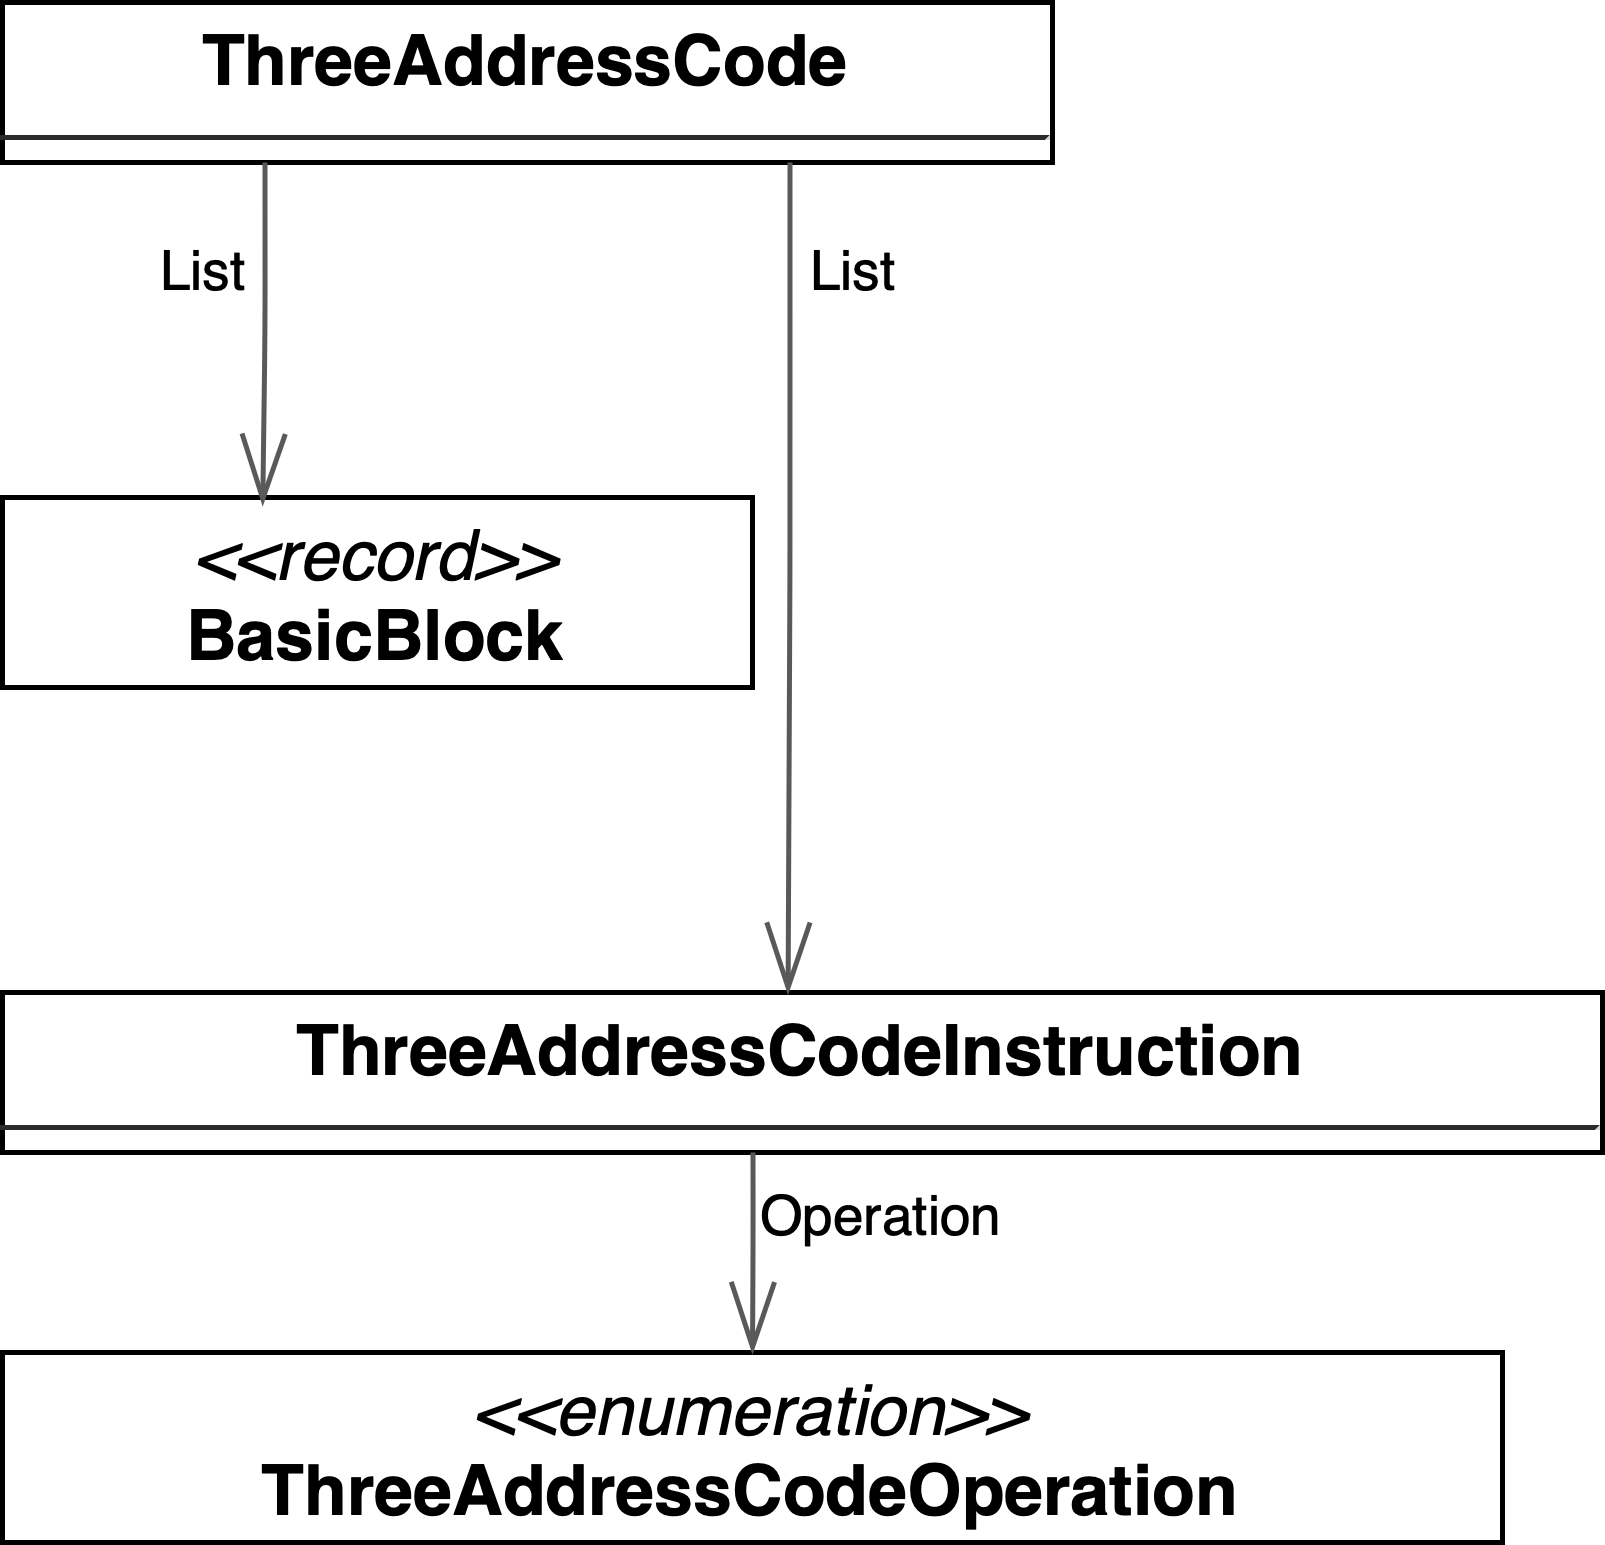
\includegraphics[width=0.5\textwidth]{fig/3AC_classes.png}
  \caption{Die Drei Address Code Klassen im Überblick}%
  \label{fig:3AC-classes}
\end{figure}


\newpage
Da der Usecase dieses Frameworks das Visualisieren von Algorithmen ist, 
braucht es folglich eine Möglichkeit, den 3-Address-Code zu visualisieren.
Hier wurde sich für eine Tabelle entschieden, da eine Instruktion in acht Zellen
\footnote{$if\ Y\ relOp\ X\ goto\ L$ ist mit 6 Elementen die längste legale 3-Address-Code Instruktion,
dazu wird noch eine Zelle für die aktuelle Instruktion und eine für Kommentare hinzugefügt.} 
aufgeteilt werden kann. Da es sich bei einem Programm immer um
eine Liste von Instruktionen handelt, ergibt sich so ein zweidimensionales Feld an Daten.
Außerdem sollen auch die Daten die wir aus unseren Analysen erheben
angezeigt werden. Auch hier ist eine Tabelle sinnvoll.\\

Um Kontrollflussgraphen anzeigen zu können, soll es ausserdem möglich sein,
Graphen anzuzeigen.\\

Mit einer Toolbar soll es möglich sein, mit dem aktuell geladenen Plugin zu interagieren.\\


Aus diesen Anforderungen ergibt sich folgendes Klassendiagramm(\cref{fig:gui-classes}):\\
\begin{figure}[h]
  \centering
  \vspace{-15pt}
  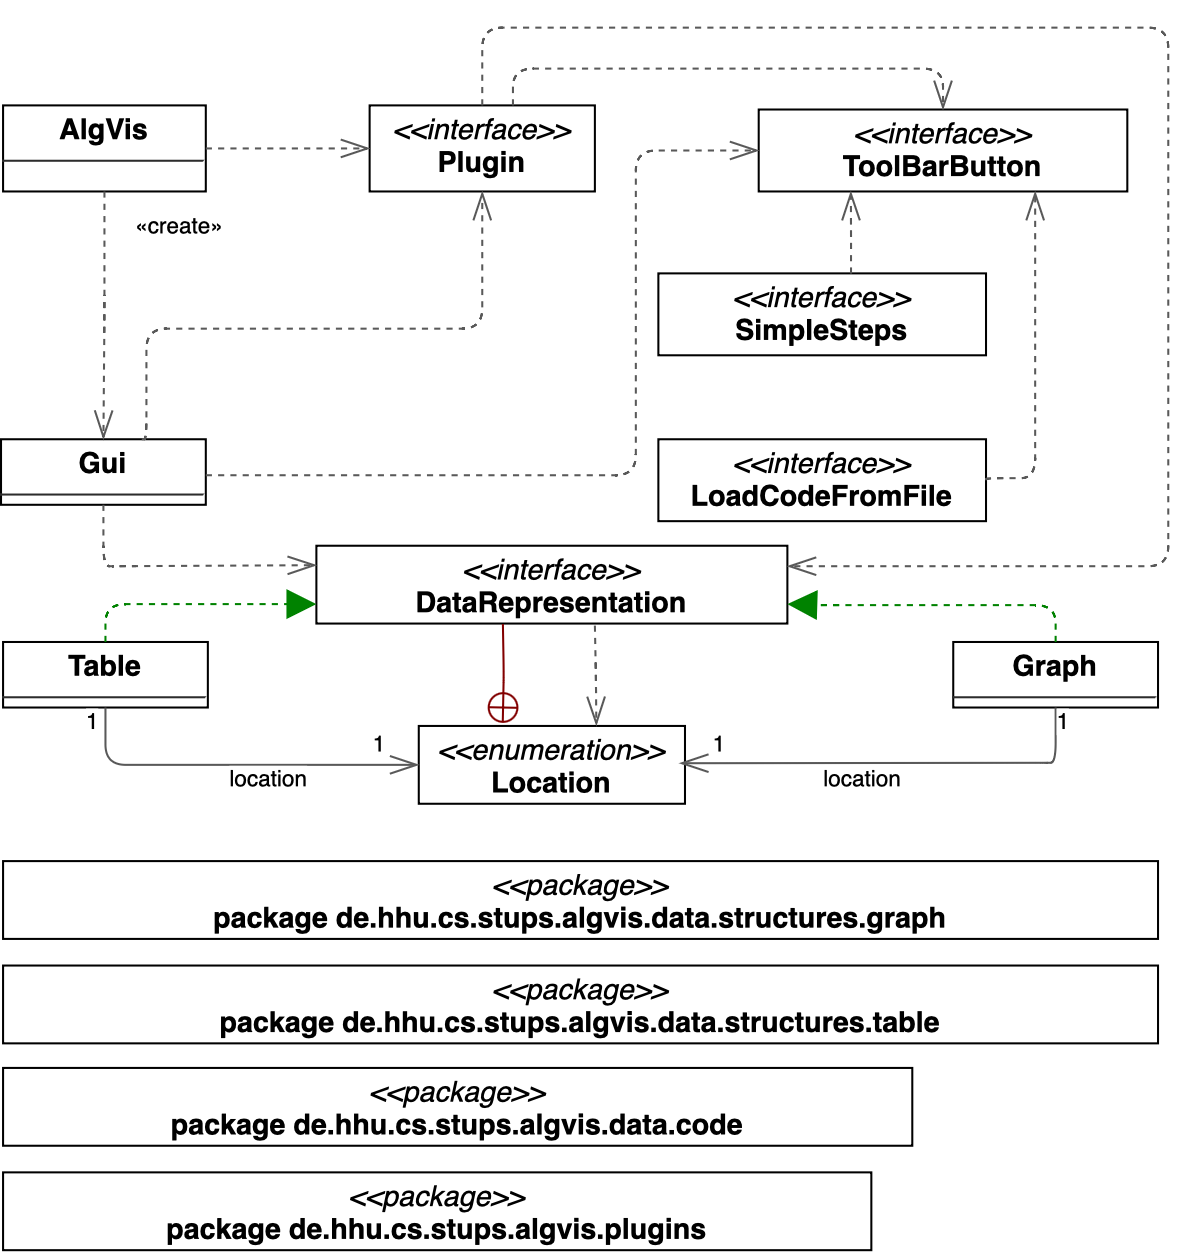
\includegraphics[width=0.75\textwidth]{fig/GUI_classes.png}
  \vspace{-10pt}
  \caption{Klassenstruktur der GUI-Klassen}%
  \label{fig:gui-classes}
\end{figure}
\vspace{-20pt}

\newpage
\begin{itemize}
  \item Die Klasse \textit{AlgVis} gilt hier (\cref{fig:gui-classes}) als Entrypoint. 
    Sie lädt alle Plugins, erstellt ein \textit{Gui} Objekt und übergibt diesem die Plugins.
  \item Das Interface \textit{Plugin} definiert, welche Methoden neue Plugins
    beziehungsweise Algorithmen
    benötigen, um hinzugefügt zu werden. Diese werden in\\
    \textit{de.hhu.cs.stups.algvis.plugins} implementiert.
  \item Zudem definiert das Interface \textit{ToolBarButton} wie Buttons der ToolBar,
    welche im nächsten Kapitel im Detail erklärt wird, implementiert werden können.
    Beispiele dafür liefern das \textit{SimpleSteps} und \textit{loadCodeFromFile} Plugin,
    welche vordefinierte Buttons anbieten.
  \item Die Packages, endend auf \textit{graph} und \textit{table} enthalten hierbei Helferklassen 
    für die jeweiligen Komponenten. Hierzu später mehr.
  \item Im Package \textit{de.hhu.cs.stups.algvis.data.code} sind die vorhin genannten Datenstrukturen
    für 3-Address-Code, Grundblöcke, 3-Address-Code-Instruktionen\\ 
    und -Operationen implementiert.
\end{itemize}

\subsection{Gui} 
Die \textit{Gui} Klasse ist das Herzstück der Visualisierung. Hier wird ein \textit{JFrame},
also ein GUI Fenster der Java Standardlibrary \textit{Swing} geladen. In ihr befinden sich
drei GUI-Elemente, auch aus der \textit{Swing}-Library:
\begin{enumerate}
  \item Eine Menüleiste, in der über ein Dropdown alle Plugins aufgerufen werden können.
  \item Ein \textit{JPanel}, welches im folgenden \textit{ContentPanel} genannt wird, 
    da sich in ihm alle grafischen Elemente des aktuell genutzten Plugins befinden.
    In ihm können Plugins Objekte die das Interface
    \textit{DataRepresentation} implementieren einfügen.
    Die Klassen \textit{Table} und \textit{Graph} implementieren dieses Interface bereits. 
    Sollte später ein Plugin eine andere Art der Darstellung benötigen,
    kann dieses das Interface mit einer anderen \textit{awt}-Komponente implementieren.
    Zum Start des Frameworks zeigt es einen SplashScreen (\cref{fig:screenshot_splashScreen}) mit dem Schriftzug \glqq welcome\grqq\ an.
  \item Und eine \textit{JToolBar}.\\
    Da die meißten Plugins ähnliche Funktionalitäten haben, wie zum Beispiel
    das schrittweise Durchlaufen eines Algorithmus, 
    wurde ein GUI-Element hinzugefügt, in dem Buttons zur Kontrolle des Plugins
    hinzugefügt werden können. Diese ist auf der Abbildung (\cref{fig:screenshot_splashScreen})
    nicht zu sehen, da aktuell kein Plugin geladen ist und somit auch kein Buttons angezeigt werden
\end{enumerate}


\newpage
\begin{figure}[h!]
  \centering
  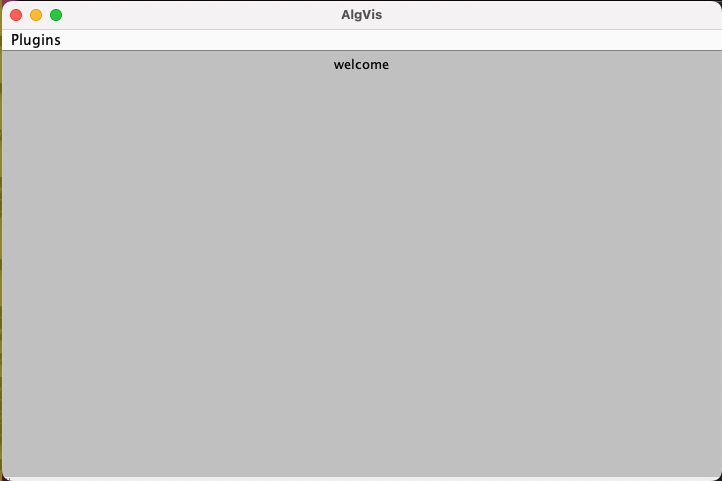
\includegraphics[width=0.7\textwidth]{fig/Screenshot_SplashScreen.png}
  \caption{Ansicht des Programmes direkt nach Start}
  \label{fig:screenshot_splashScreen}
\end{figure}



\subsection{Darstellen von Daten}
\begin{wrapfigure}[10]{r}{0.3\textwidth}
  \vspace{-15pt}
  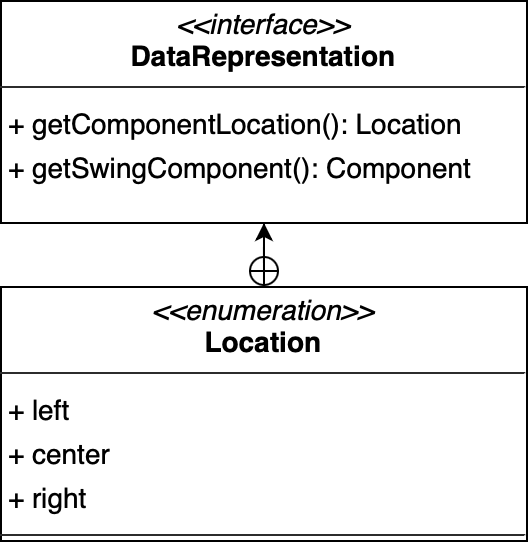
\includegraphics[width=0.3\textwidth,]{fig/GUI_DataRepresentation.png}
  \vspace{-15pt}
  \caption{Das DataRepresentation Interface und sein Location enum}
  \label{fig:DataRepresentation}
  \vspace{-30pt}
\end{wrapfigure}
Um grafische Elemente im \textit{ContentPanel} darzustellen wird das Interface \textit{DataRepresentation}
von Gui-Klassen implementert. Dadurch kann auf zwei Methoden zugegriffen werden:
\begin{itemize}
  \item \textit{getSwingComponent()} gibt die \textit{awt}-Komponente zurück, welche dem \textit{ContentPanel}
    hinzugefügt wird.
\item Durch die Methode \textit{getComponentLocation()} wird bestimmt an welcher
  Position im \textit{ContentPanel} diese angezeigt wird.
  Das Enum \textit{Location} entscheidet hierbei wo im \textit{ContentPanel} das Gui-Objekt
  angezeigt wird.

\end{itemize}





Für diese Arbeit wurden folgende Gui-Klassen implementiert:


\newpage
\subsubsection{Graphen}
\begin{wrapfigure}{r}{0.17\textwidth}
  \vspace{-10pt}
  \centering
  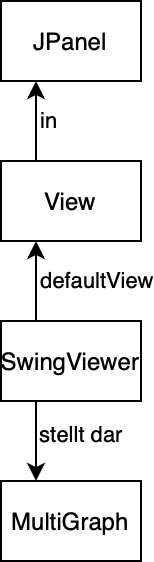
\includegraphics[width=0.1375\textwidth]{fig/GUI_Graph_rendering_pipeline.png}
  \caption{Rendering Pipeline eines Graphen}%
  \label{fig:graph-rendering-pipeline}
  \vspace{-10pt}
\end{wrapfigure}
Graphen werden durch die Klasse \textit{Graph} und zwei Subklassen 
\textit{Edge} und \textit{Node} realisiert (siehe \cref{fig:graph-classes}).
Da das Schreiben einer eigenen Engine für die Darstellung von Graphen
diese Bachelorarbeit übertreffen würde, wurde entschieden, eine externe Library
zu verwenden. Hier wurde sich für GraphStream \cite{GS}
entschieden.\\

Graphstream ist eine Library zum modellieren, analysieren und visualisieren von Graphen,
im Framework wird sie jedoch nur benutzt um Graphen zu visualisieren.\\
Um einen Graphen im \textit{ContentPanel} anzeigen zu lassen, gibt 
die Methode \textit{getSwingComponent()} ein JPanel wieder. 
In diesem JPanel befindet sich ein GraphStream \textit{View} Objekt, welches von einem
\textit{SwingViewer} erstellt wird, welcher in einem eigenen Thread (siehe \cref{cde:graph-constructor}) einen
\textit{MultiGraph} rendert (siehe \cref{fig:graph-rendering-pipeline}).
Dies stellt die default Renderingstrategie dar \cite{GS_render}.\\
Graphstream bietet einige verschiedene Implementierungen von Graphen an, 
die je nach Usecase unterschiedliche Vorteile haben. Hier wurde sich dafür
entschieden nur die \textit{MultiGraph} Implementierung zu verwenden, da es
möglich sein muss mehrere Kanten zwischen denselben zwei Knoten zu haben.
\footnote{Es wird die Möglichkeit benötigt, eine Kante a>b und eine Kante b>a gleichzeitig darzustellen}
Diese Implementierung wird laut Dokumentation nur von einem \textit{MultiGraph}
umgesetzt.\cite{GS_graphs}\\

Nun wird im GUI ein leerer Graph angezeigt.\\
Um dem \textit{MultiGraph} nun einen Knoten hinzuzufügen, benutzen wir 
die Methode \textit{addNode(String)}. Diese erwartet einen String als ID,
dementsprechen müssen alle Knoten, die wir hinzufügen einen eindeutigen
String haben.\\
Um eine Kante hinzuzufügen, wird die Methode \textit{addEdge(String, String, String, boolean)} verwendet.
Hierbei soll der erste String die eindeutige ID der Kante sein und die beiden folgenden Strings
die IDs der jeweiligen Aus- und Eingangsknoten.
Der Boolean-Wert gibt hierbei an, ob die Kante eine gerichtete Kante ist oder nicht.
Um Knoten oder Kanten zu entfernen gibt es die Methoden \textit{removeNode(String)},
und \textit{removeEdge(String)} die nach demselben Prinzip agieren.\\

Um das Aussehen eines Graphen anzupassen werden Attribute benutzt \cite{GS_data}.
Attribute können Graphen, Knoten und Kanten mit der Methode \textit{setAttribute(String, Object)}
hinzugefügt werden, hierbei ist der erste String das Attribut und das folgende
Objekt der Wert des Attributes. Im Falle dieser Arbeit sind zwei Attribute relevant:
\begin{itemize}
  \item Das generelle \glqq look and feel\grqq\ des Graphen wird durch das \glqq ui.stylesheet\grqq\ 
    Attribut bestimmt. Dieses setzen wir für das Graph-Objekt mit\\
    \textit{graph.setAttribute(\glqq ui.stylesheet\grqq, \glqq [...]\grqq)}
  \item Um die einzelnen Knoten von einander unterscheiden zu können, gibt es
    die Möglichkeit, diese mit einem Text zu versehen. Das Attribut hierfür ist
    \glqq ui.label\grqq . Um einem Knoten ein Label zu geben, ist unser Methodenaufruf folglich\\
    \textit{node.setAttribute(\glqq ui.label\grqq, \glqq [...]\grqq)}. Da wir diese Methode auf einem 
    node-Objekt aufrufen, dies aber nicht selber erstellen, benötigen wir ausserdem
    die Methode \textit{graph.getNode(String)}, bei der der übergebene String
    wieder die ID des Knotens ist.
\end{itemize}


Um unabhängig von \textit{GraphStream} mit Graphen umzugehen zu können, wurde mit
folgender (\cref{fig:graph-classes}) Abstraktion gearbeitet:\\
\begin{figure}[h]
  \centering
  \vspace{-20pt}
  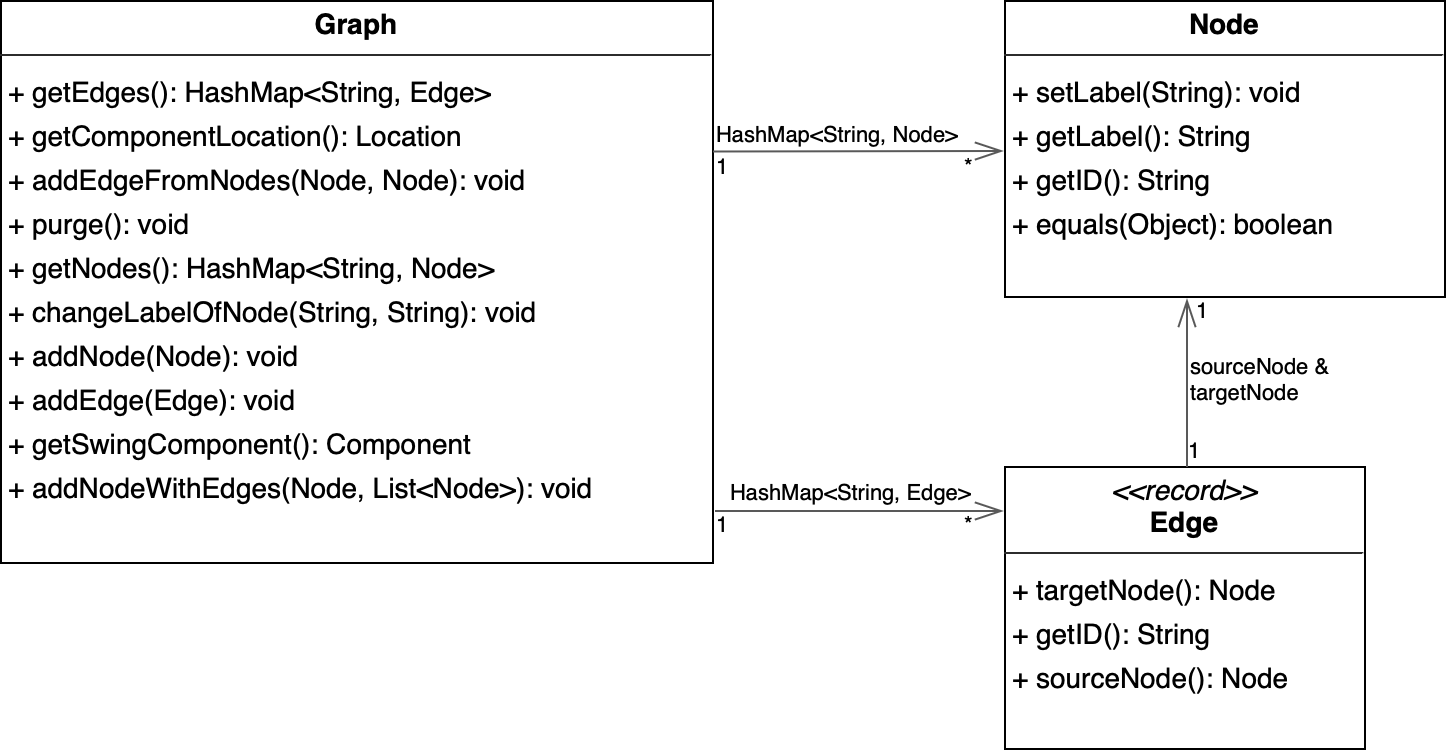
\includegraphics[width=0.99\textwidth]{fig/GUI_Graph_classes_methods.png}
  \caption{Klassenstruktur der Graph-Klassen}%
  \label{fig:graph-classes}
\end{figure}


Hierbei sind die Klassen \textit{Node} und \textit{Edge} Helferklassen, um
anstelle von Strings mit Node- beziehungsweise Edge-Objekten zu arbeiten.\\
Einem \textit{Node}-Objekt wird zu ihrer Erstellung eine eindeutige ID zugewiesen,
um das Objekt später mit in einem \textit{GraphStream}-Graphen verwenden zu können.\\
Ein \textit{Edge}-Objekt ist ein Record, welcher zwei Node-Objekte
sourceNode und targetNode referenziert. Die für \textit{GraphStream}
eindeutige ID bestimmt sich dann durch die \textit{getID()}-Methode(\cref{cde:edge-id}):

Die \textit{Graph} Klasse ist die zentrale Klasse für die Visualisierung von Graphen.
Sie implementiert das \textit{DataRepresentation} Interface und
alle nötige Kommunikation mit der \textit{GraphStream} Library.

Die im Graph enthaltenen Knoten und Kanten werden in einem \textit{Set} gespeichert (\cref{cde:graph-constructor}),
wenn ein Plugin dem Graphen einen Knoten hinzufügen möchte,
ruft er die Methode \textit{addNode(Node)}(\cref{cde:graph-addNode}) auf.
Diese fügt den Knoten dem Set der im Graphen enthaltenen Knoten hinzu und
fügt dem Graphen einen neuen Knoten mit der ID des übergebenen Knotens hinzu.
Anschließend wird die Methode \textit{layout.shake()} aufgerufen.
diese Methode sorgt dafür, dass die Anordnung der Knoten neu berechnet wird,
sodass diese immer einen angemessenen Abstand zu einander haben und sich nicht überlappen. 
Analog gibt es auch die Methode \textit{addEdge(Edge)}, um Kanten hinzuzufügen
und die Methoden \textit{removeEdge(Edge)} und \textit{removeNode(Node)}
um diese wieder zu entfernen.\\
Um den Graphen komplett zu leeren, wurde die Methode \textit{purge()} hinzugefügt.
diese entfernt alle Knoten und Kanten vom Graphen.\\
Um einem Knoten ein Label zu geben, wurde die Methode\\
\textit{setLabelOfNode(Node, String)}(\cref{cde:graph-labelNode})hinzugefügt.

\subsubsection{Tabellen}
\begin{wrapfigure}[15]{r}{0.4\textwidth}
  \centering
  \vspace{-20pt}
  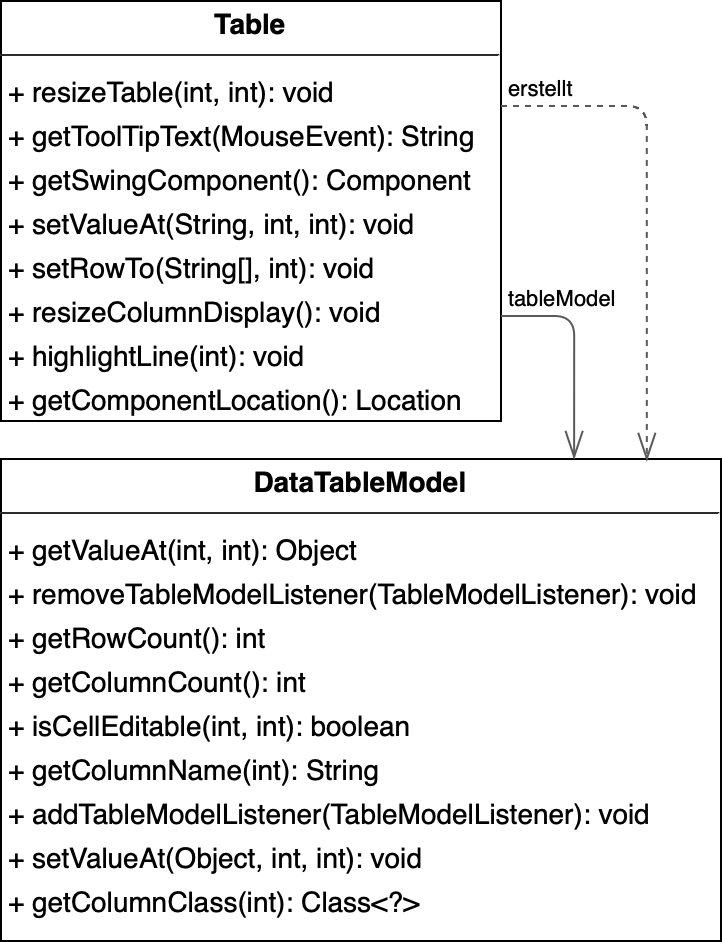
\includegraphics[width=0.33\textwidth]{fig/GUI_Table_classes.png}
  \caption{Klassenstruktur der Tabellenvisualisierung}
  \label{fig:table-classes}
  \vspace{-20pt}
\end{wrapfigure}

Tabellen werden durch die Klasse \textit{Table} (\cref{fig:table-classes}) visualisiert. Da bereits
mit der \textit{JTable} von der \textit{swing}-Library eine
Tabellenvisualisierung angeboten wird, wurde diese auch implementiert.\\
Ein \textit{JTable}-Objekt benötigt immer ein \textit{TableModel}, welches
die Daten, welche dargestellt werden sollen enthält.\\
Dieses wird von der Klasse \textit{DataTableModel} (\cref{fig:table-classes}) implementiert.
Sie speichert die Daten in einem zweidimensionalen String-Array und implementiert
alle vom \textit{TableModel}-Interface vorgegebenen Methoden.

Die notwendigen, nicht trivialen Methoden wurden wie folgt implementiert:
\begin{itemize}
  \item \textit{isCellEditable(int, int)} gibt immer \textit{false} zurück,
    da es nicht erwünscht ist, dass der Benutzer die Tabelle bearbeiten kann.
    Ein Plugin kann die Tabelle trotzdem bearbeiten.
  \item Die Methode \textit{getColumnName(int)} gibt immer \textit{null} zurück,
    da in aktuellen Stand des Frameworks Überschriften selber gesetzt werden.
  \item Die Methoden \textit{addTableModeListener(TableModelListener)} und
    \textit{removeTableModeListener(TableModelListener)} fügen eine Implementation
    der Klasse TableModelListener einer zugehörigen Liste hinzu, beziehungsweise
    entfernen sie
    \footnote{Diese Funktionalität ist notwendig, da das \textit{JTable}-Objekt sich als Listener hinzufügt.}.
  \item \textit{setValueAt(Object, int, int)} versucht den Wert am übergebenen Index
    zu überschreiben. Wenn dies möglich ist werden alle
    Objekte in der TableModelListener Liste benachrichtigt (\cref{cde:setValueAt}).
\end{itemize}


Ein Objekt der \textit{Table}-Klasse (\cref{fig:table-classes}) erweitert die
von \textit{swing} gegebene \textit{JFrame}-Klasse und gibt sich selber in 
\textit{getSwingComponent()} zurück.

Die für Plugins verfügbar gestellten Methoden sind:
\begin{itemize}
  \item Die Methode \textit{resizeTable(int, int)} (\cref{cde:resizeTable}) erstellt ein neues
    \textit{DataTableModel}-Objekt mit der spezifizierten Größe und setzt dieses
    als neues \textit{TableModel}.
  \item \textit{setValueAt(String, int, int)} setzt den übergebenen String
    als Wert an der übergebenen Position, indem es \textit{setValueAt(Object, int, int)}
    im \textit{DataTableModel} aufruft.
  \item \textit{setRowTo(String[], int)}
    setzt die Werte für eine gesamte Zeile indem es über das String-Array iteriert.
  \item \textit{highlightLine(int)} (\cref{cde:highlightLine})
    markiert die übergebene Zeile.
\end{itemize}

Desweiteren wurden zwei weitere Funktionen implementiert, um Zelleninhalte
besser zu visualisieren:\\
\begin{itemize}
  \item Die Methode \textit{getToolTipText(MouseEvent)} (siehe \cref{cde:tooltip}) überschreibt die in \textit{JTable}
    definierte Methode. Sie erwirkt, dass wenn der Benutzer seine Maus auf eine
    Zelle bewegt, der Inhalt dieser Zelle als ToolTip angezeigt wird. Dies ist gerade dann
    sinnvoll, wenn die Zelle zu klein für ihren Inhalt ist.\\
  \item Die Methode \textit{resizeColumnDisplay()} (siehe \cref{cde:resize}) versucht, jeder Spalte die
    kleinstmögliche Breite zu geben und den übrigen Platz auf die letzte Spalte aufzuteilen.
    Dies ist, wenn wir 3-Address-Code darstellen wollen, sehr sinnvoll, da in der letzten Spalte der Kommentar steht.
\end{itemize}



\newpage
\subsection{Drei Address Code}
Im folgenden Kapitel wird die Implementierung des drei Address Codes erläutert.
Wie zu Beginn von \cref{tac} angeführt, werden diese Klassen benötigt:
\begin{figure}[h]
  \centering
  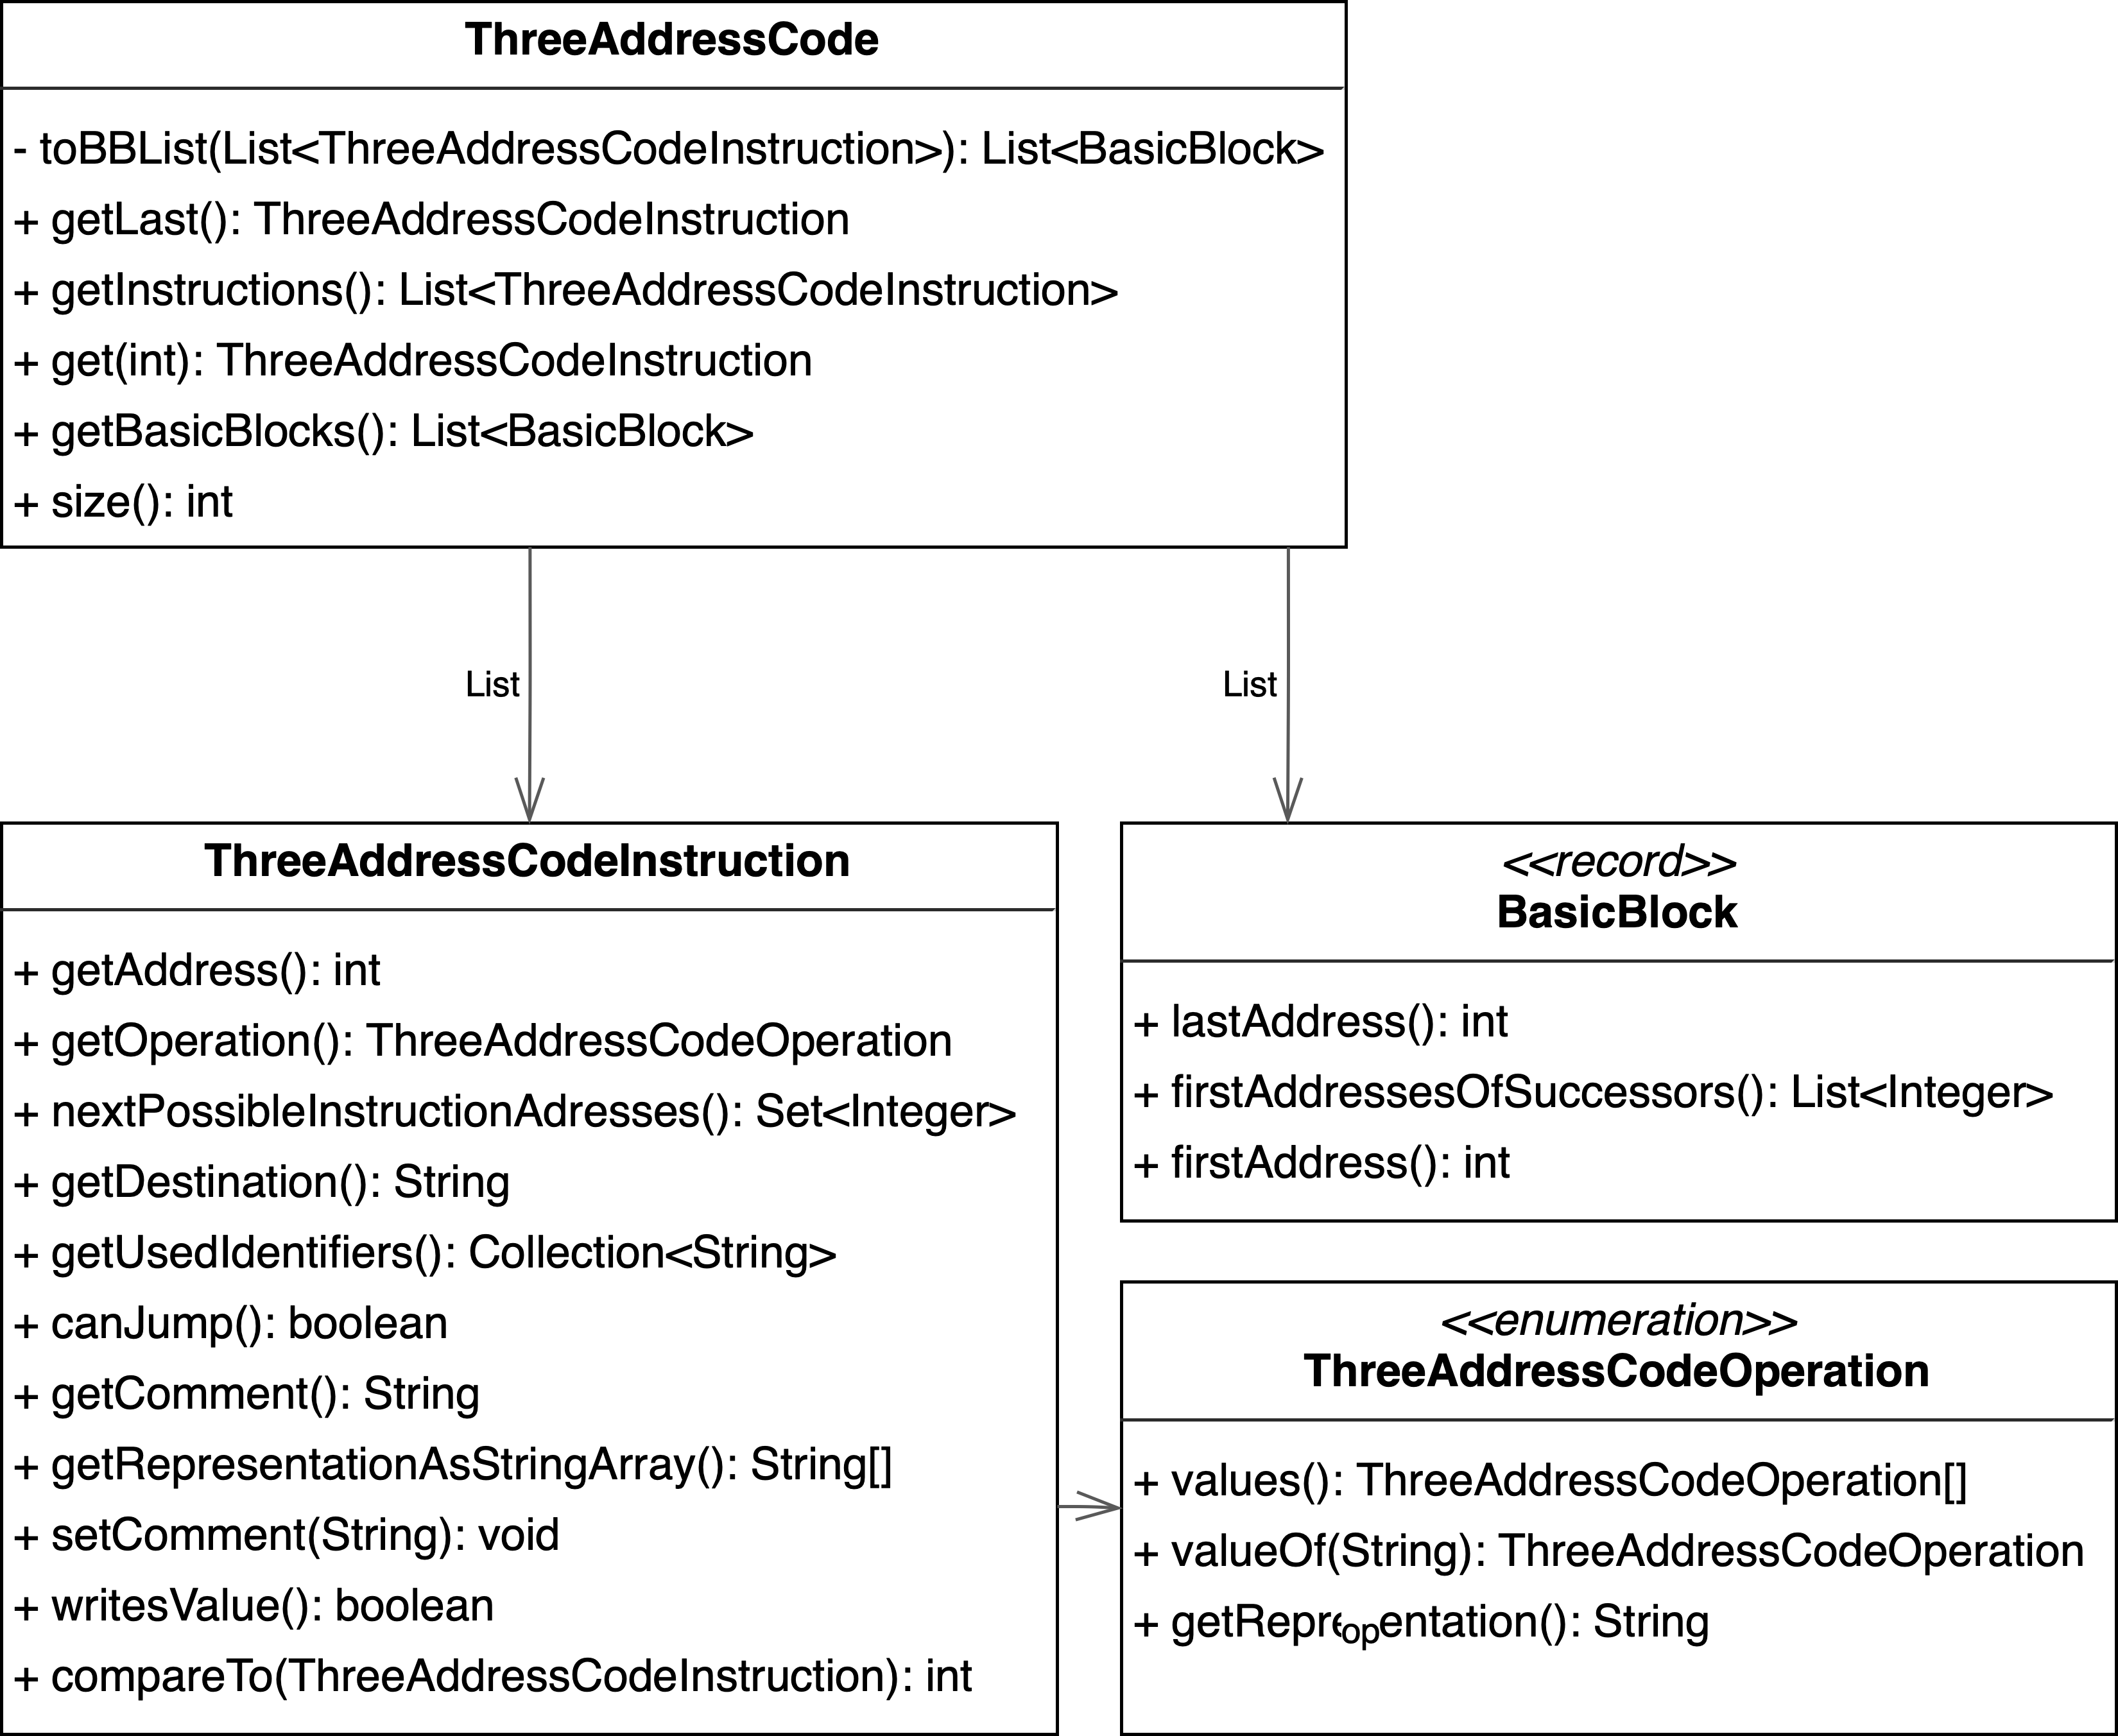
\includegraphics[width=0.98\textwidth]{fig/3AC_classes_methods.png}
  \caption{Implementation der drei Address Code Klassen}
  \label{fig:3ac-classes}
\end{figure}


\newpage
\subsubsection{Die ThreeAddressCodeInstruction Klasse}
\begin{wrapfigure}{r}{0.33\textwidth}
  \centering
  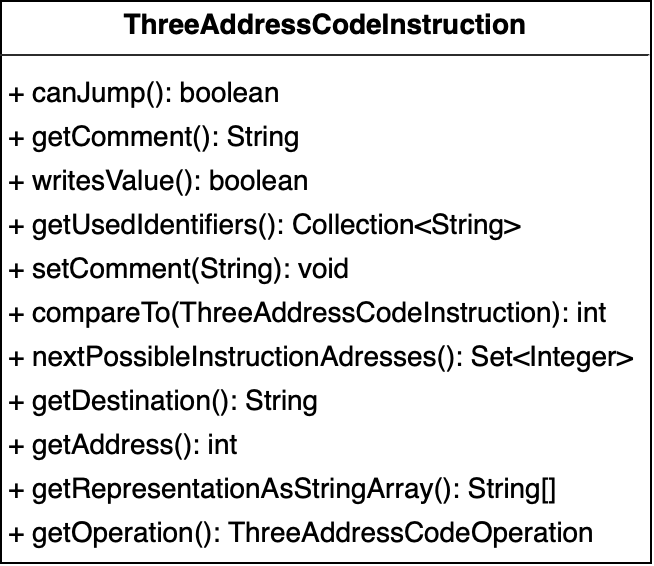
\includegraphics[width=0.4\textwidth]{fig/3AC_ThreeAddressCodeInstruction_methods.png}
  \caption{Die ThreeAddressCodeInstruction Klasse}
  \label{fig:ThreeAddressCodeInstruction}
\end{wrapfigure}

Um einzelne Instruktionen zu modellieren, wird die Klasse 
\textit{ThreeAddressCodeInstruction} verwendet.
Generiert werden diese aus einem String und einer Zahl, nämlich der
Adresse an der Stelle ihres Programms.
Dies ist zwar streng gesehen eine Ungenauigkeit der Modellierung, 
da jede Instruktion zwar eine Adresse hat, 
diese jedoch nicht in Bezug direkt auf die einzelne Instruktion steht,
sondern nur im Kontext des Gesamtprogrammes gesehen werden kann.\\
Da es jedoch die Implementierung einiger folgender Methoden stark vereinfacht
und keine Instruktion ohne eindeutige Adresse an der sie gespeichert oder ausgeführt werden kann
existiert, wurde sich dazu entschieden, für diese ein Attribut anzulegen.\\

Um die in \cref{t:tac} definierten Instruktionen zu modellieren, werden folgende
weitere Attribute benötigt:
\begin{enumerate}
  \item Eine \textit{ThreeAddressCodeOperation}. Dies ist ein Enum, welches definiert
    welche Operation die angegebene Instruktion ausführt.
  \item Ein String namens \textit{destination}. Dieser gibt entweder das Ziel eines Sprunges an,
    oder den Ort, an dem eine Berechnung gespeichert werden soll.
  \item Den String \textit{source}. Da alle Instruktionen ausser dem unbedingten Sprung
    mindestens einen Wert verarbeiten.
  \item Und einen String \textit{modifier}, für Instruktionen, die zwei Werte
    entweder vergleichen oder arithmetisch verrechnen.
\end{enumerate}
Desweiteren wurde ein weiteres String-Attribut \textit{comment} zum Speichern von Kommentaren
hinzugefügt.

Um aus dem Eingabestring ein passendes \textit{ThreeAddressCodeInstruction}-Objekt
zu generieren, wird der Eingabestring im Konstruktor (\cref{cde:taci-constructor})
in seine Bestandteile aufgelöst und der richtigen Instruktion zugeordnet.

\newpage
Außerdem wurden folgende Helfermethoden, welche im späteren Verlauf dieser Arbeit
benötigt werden, implementiert:
\begin{enumerate}
  \item Die Methode \textit{canJump()} gibt den Wahrheitswert $wahr$ zurück, wenn die
    Instruktion springen kann oder immer springt, ansonsten gibt sie $falsch$ zurück.
  \item Die Methode \textit{writesValue()} gibt den Wahrheitswert $wahr$ zurück,
    wenn die Instruktion den Wert, der in \textit{destination} gespeichert ist überschreibt.
    Ansonsten gibt sie $falsch$ zurück.
  \item \textit{getUsedIdentifiers()} gibt die Menge der Werte in \textit{source} und \textit{modifier} zurück,
    wenn diese Variablen referenzieren und keine Konstanten sind.
  \item Die Methode \textit{compareTo(ThreeAddressCodeInstruction)} implementiert das Interface
    Comparable<>. Wir sehen später dass dies sinnvoll ist wenn in Erfahrung gebracht werden
    soll sich ob zwei Instruktionen im selben Grundblock befinden.
  \item \textit{nextPossibleInstructionAddresses()} gibt die Menge der nächsten möglichen 
    Instruktionsadressen zurück. Dies ist in den meisten Fällen einfach die nächste
    Adresse, wenn die aktuelle Instruktion jedoch ein unbedingter Sprung ist, ist es der
    Wert in \textit{destination}. Wenn die Instruktion ein bedingter Sprung ist, wird sowohl die
    nächste Adresse als auch der Wert in \textit{destination} zurückgegeben.
  \item Die Methode \textit{getRepresentationAsStringArray()} gibt
    eine Repräsenationen der Instruktion als \textit{String[]} in der Form zurück, 
    dass die Elemente des Arrays nacheinander die eingelesene Instruktion bilden.
\end{enumerate}
Die restlichen in \textit{ThreeAddressCodeInstruction} enthaltenen Klassen sind getter und setter Methoden.

\subsubsection{Die BasicBlock Record-Klasse}
\begin{wrapfigure}{r}{0.35\textwidth}
  \vspace{-15pt}
  \centering
  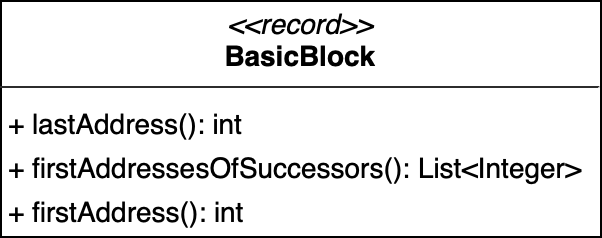
\includegraphics[width=0.35\textwidth]{fig/3AC_BasicBlock_methods.png}
  \caption{Die ThreeAddressCodeInstruction Klasse}
  \label{fig:BasicBlock}
\end{wrapfigure}
Um die Grundblöcke eines Programms zu modellieren, reicht uns eine Record-Klasse.
Da Grundblöcke immer ein gesamtes Programm partitionieren, reicht es, die erste und 
letzte der enthaltenen und die Menge der folgenden Adressen zu kennen.\\


\newpage
\subsubsection{Die ThreeAddressCode Klasse}
\begin{wrapfigure}{r}{0.4\textwidth}
  \vspace{-15pt}
  \centering
  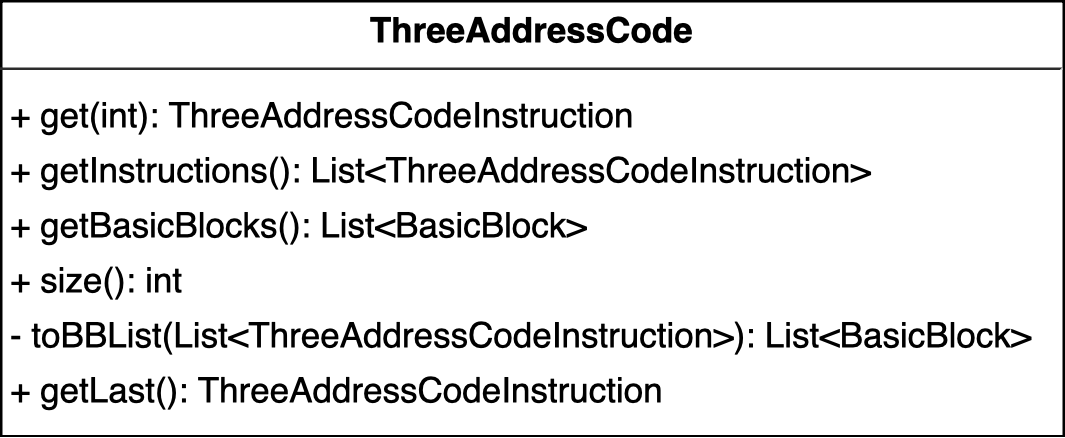
\includegraphics[width=0.4\textwidth]{fig/3AC_class_methods.png}
  \caption{Die ThreeAddressCode Klasse}
  \label{fig:ThreeAddressCode}
\end{wrapfigure}

Die Klasse \textit{ThreeAddressCode} agiert im Framework als Modellierung eines
gesamten Programmes. Ihr Konstruktor (\cref{cde:tac-constructor}) wird mit
einem String aus 3-Address-Code Instruktionen welche durch einen Zeilenumbruch getrennt sind
aufgerufen. Daraus generiert sie eine Liste and \textit{ThreeAddressCodeInstruction}
Objekten und aus diesen Objekten wiederum eine Liste an \textit{BasicBlock} Objekten.

Die Methode \textit{toBBList(List<ThreeAddressCodeInstruction>)} ist hier eine statische Methode, welche für eine
Liste an \textit{ThreeAddressCodeInstruction}-Objekten eine Liste an \textit{BasicBlock}-Objekten
zurückgibt. Dafür wurde der in \cref{t:bb} angegebene Algorithmus implementiert (\cref{cde:bb-gen}).
In Folge dessen werden die nächstmöglichen Instruktionsadressen bestimmt.

Um alle Leader zu finden wurde wie folgt über die Instruktionsliste iteriert(\cref{cde:bb-leader}).
Wenn die Instruktion an der Stelle i springen kann, ist das Ziel des Sprungs ein Leader.\\
Ausserdem ist die Instruktion an der Stelle i+1 auch ein Leader, wenn sie existiert
Um die ersten Adressen der Nachfolger zu erhalten, schauen wir uns die letzte
Adresse unseres Blockes an(\cref{cde:bb-successor}), da an dieser entweder ein Sprung ist,
an die nächste Adresse gesprungen wird oder das Programm zuende ist.
Mit diesen Klassen und Methoden wurden alle für die Implementation der Plugins
notwendigen Modellierungen abgebildet. 


\newpage
\subsection{Implementierung von Algorithmen}
\begin{wrapfigure}[18]{r}{0.475\textwidth}
  \centering
  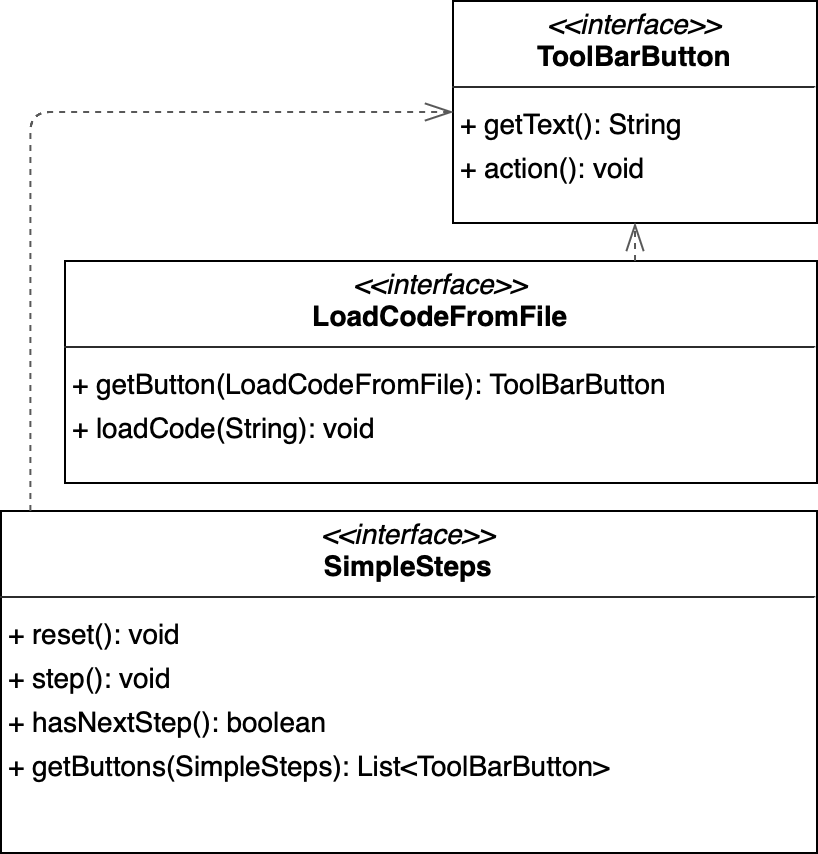
\includegraphics[width=0.47\textwidth]{fig/GUI_ToolBar_classes_methods.png}
  \caption{Das ToolBarButton Interface}
  \label{fig:ToolBarButtons}
\end{wrapfigure}


Dieser Abschnitt befasst sich damit, wie Algorithmen als Plugins implementiert werden,
sodass diese vom Framweork richtig visualisiert werden.

Hierbei gibt es zwei Interfaces die implementiert wurden, das \textit{Plugin} Interface
und das \textit{ToolBarButton} Interface.
Letzteres spezifiziert alle Buttons, welche in der Toolbar angezeigt werden, 
wenn das Plugin geladen ist. Es ist sehr einfach aufgebaut und verfügt nur über zwei Methoden.
Eine Methode \textit{getText()} gibt einen String zurück, welcher im Button angezeigt wird.
Die andere Methode \textit{action()} wird ausgeführt, wenn der Nutzer auf den zugehörigen Button drückt.\\
Da alle in dieser Arbeit implementierten Algorithmen sowohl schrittweise durchlaufen werden
sollen, als auch Code laden müssen wurden außerdem zwei Interfaces implementiert, 
welche \textit{ToolBarButtons} für Plugins bereitstellen.

Das Interface \textit{LoadCodeFromFile} stellt sicher, dass es eine Funktion \textit{loadCode(String)}
gibt, in die Code als ein String in das Plugin geladen werden kann.\\
Die Funktion \textit{getButton()} ist hier eine statische Funktion, welche eine Implementation
von \textit{ToolBarButton} zurückgibt welche zuerst einen \textit{JFileChooser}
\footnote{\textit{JFileChooser} ist eine Klasse aus der \textit{swing}-Library welche eine Bedienfläche zum öffnen von Dateien bietet}
öffnet und dann die Datei als String lädt. Hierbei wird auch der Unterschied
zwischen Windows und *nix basierenden Systemem berücksichtigt und die einzelnen
Zeilen nur mit einem Zeilenumbruch(\textbackslash n)getrennt.

Das Interface \textit{SimpleSteps} implementiert sogar drei Buttons und somit auch
drei Methoden. Ein Reset Button, der die Methode \textit{reset()} aufruft, ein Step
Button, der die Methode \textit{step()} aufruft und ein Run Button, der die Methode
\textit{step()} so lange aufruft, wie die Methode \textit{hasNextStep() wahr} zurückgibt.
Diese drei Buttons werden wieder in einer statischen Funktion \textit{getButtons()}
generiert.\\


\newpage
\subsubsection{Das Plugin Interface}
\begin{wrapfigure}[4]{r}{0.5\textwidth}
  \centering
  \vspace{-20pt}
  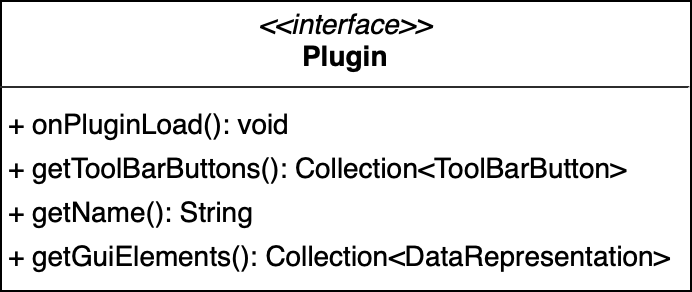
\includegraphics[width=0.46\textwidth]{fig/Plugin_methods.png}
  \caption{Das Plugin Interface}
  \label{fig:PluginInterface}
  \vspace{-20pt}
\end{wrapfigure}

Das \textit{Plugin} Interface (\cref{fig:PluginInterface}) beschreibt die
Schnittstelle zwischen dem Framework und dem entwickelten Plugin.
Um ein Plugin zu implementieren, benötigt es folgende Methoden:
\vspace{30pt}

\begin{itemize}
  \item \textit{onPluginLoad()} wird ausgeführt, wenn das Plugin geladen wird also zum 
    Beispiel, wenn der Nutzer im Plugin Dropdown Menü auf den Button mit dem Namen des
    Plugins drückt.
  \item \textit{getToolBarButtons()} gibt eine Collection der implementierten \textit{ToolBarButtons}
    zurück, sodass diese, wenn das Plugin geladen wird, in die ToolBar eingefügt werden.
  \item \textit{getName()} gibt den Namen des Plugins zurück, sodass er im Plugin Dropddown Menü
    angezeigt wird.
  \item \textit{getGuiElements()} gibt eine Collection der \textit{DataRepresentation} Elemente
    zurück, die das Plugin anzeigen soll.
\end{itemize}
Mehr Abstraktionen braucht das Framework nicht um alle Algorithmen die in dieser
Arbeit implementiert werden sollten zu visualisieren.
Im nächsten Kapitel wird nun auf die spezifische Implementationen der Algorithmen eingegangen.

\newpage
%! TeX root: thesis.tex
\section{Implementierte Algorithmen}
Die folgenden Kapitel behandeln die Implementation der in Kapitel 1.2 vorgestellten
Algorithmen.

Sämtliche Algorithmen wurden nach folgendem Muster implementiert:
Es gibt eine Hauptklasse, die das \textit{Plugin} Interface, das 
\textit{SimpleSteps} Interface und das \textit{loadCodeFromFile} Interface 
implementiert und eine zweite Klasse, welche den Durchlauf eines Algorithmus
Modelliert. Dies bedeutet, dass einige Methoden fast identisch implementiert wurden:

\begin{itemize}
  \item \textit{getName()} gibt den Namen des Plugins zurück.

  \item Die Methode \textit{getToolBarButtons()} gibt eine Collection der Buttons zurück,
    die in den statischen Methoden der jeweils implementierten Interfaces 
    \textit{SimpleSteps} und \textit{loadCodeFromFile} generiert werden.

  \item \textit{getGuiElements()} gibt eine Collection der Gui-Elemente zurück.
    Welche Gui-Elemente genau zurückgegeben werden und an welcher Position diese
    sind, unterscheidet sich allerdings von Plugin zu Plugin.

  \item Die \textit{onPluginLoad()}-Methode (siehe \cref{fig:PluginInterface}) 
    setzt das Plugin zurück, indem es die \textit{reset()}-Methode aufruft.
    Da alle Plugins \textit{SimpleSteps} (siehe \cref{fig:ToolBarButtons}) implementieren,
    ist es für den Benutzer am intuitivsten, wenn der geladene Algorithmus sich zwar
    zurücksetzt, aber trotzdem den geladenen Code behält.

  \item \textit{loadCode(String)} ersetzt den aktuell geladenen Code, welcher im Attribut
    \textit{currentlyLoadedCode} gespeichert ist und führt dann auch die 
    \textit{reset()}-Methode aus.

  \item Die Methode \textit{step()} führt eine gleichnamige Methode in der
    Algorithmus ausführenden Klasse auf und aktualisiert dann die Gui-Elemente, 
    indem es die Methode \textit{refreshGuiElements()} ausführt.

  \item \textit{hasNextStep()} gibt den negierten Wahrheitswert der Methode 
    \textit{isFinished()} der Algorithmusklasse zurück.

  \item Die \textit{reset()} Methode generiert ein neues Objekt der zugehörigen
    Algorithmusklasse mit dem aktuell geladenen Code, setzt dann die 
    Gui-Elemente zurück und initialisiert diese dann erneut.
\end{itemize}


Zudem hat jede \textit{Plugin}-Klasse eine \textit{refreshGuiElements()}-Methode,
in der das Gui aktualisiert wird. Diese ist nicht Teil des Interfaces, da
das Framework nicht darauf zugreift. Da das Gui jedoch sowohl beim Laden des Plugins, 
als auch beim Zurücksetzen und Durchschreiten des Algorithmusses aktualisiert werden muss,
spart dies Codeduplizierungen ein.






\subsection{Erstellung von Grundblöcken aus 3-Address-Code}
\begin{figure}[h]
  \centering
  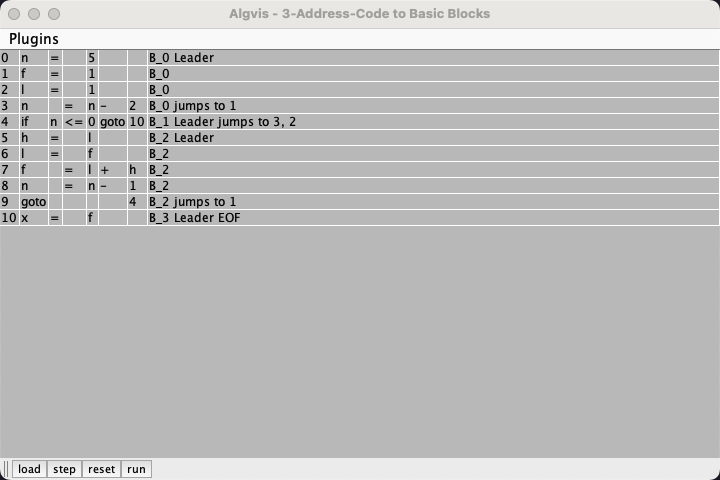
\includegraphics[width=0.8\textwidth]{fig/Screenshot_TacToBb.png}
  \caption{Das "3-Address-Code zu Grundblöcken" Plugin}
  \label{sc:TACtoBB}
\end{figure}
Dieses Plugin implementiert den in \cref{t:bb} eingeführten Algorithmus
und zeigt das 3-Address-Code Programm in einer Tabelle an (\cref{sc:TACtoBB}). Nach der
Ausführung des Programms wird in der Kommentarspalte der Tabelle für jede
Instruktion angezeigt zu welchem Grundblock sie gehört. Zudem wird auch angezeigt,
welche die folgenden Grundblöcke für jeden einzelnen Grundblock sind.

Dafür wird beim Erstellen eines Objektes der Algorithmusklasse 3-Address-Code
als String übergeben, ein \textit{ThreeAddressCode}-Objekt und ein Set erstellt, 
in welchem die gefundenen Leader gespeichert werden.

Durch das Aufrufen der \textit{step()}-Methode wird nun zwei Mal durch die
Instruktionen des \textit{ThreeAddressCode}-Objekts iteriert.

\newpage
Im ersten Durchlauf werden alle Leader markiert (\cref{cde:markLeaders}):
\begin{lstlisting}[language=Java, caption={Markieren von Leadern}, label={cde:markLeaders}]
ThreeAddressCodeInstruction instruction = code.get(address);
if(instruction.canJump()) {
  ThreeAddressCodeInstruction destination = code.get(
    Integer.parseInt(instruction.getDestination())
  );
  leaders.add(destination);
  destination.setComment("Leader");
  if(address+1 < code.size() 
  && instruction.getOperation() != ThreeAddressCodeOperation.jmp) {
    ThreeAddressCodeInstruction nextInstruction = code.get(address + 1);
    leaders.add(nextInstruction);
    nextInstruction.setComment("Leader");
  }
}
\end{lstlisting}

Im zweiten Durchlauf werden alle Instruktionen ihrem Block zugeordnet:
\begin{lstlisting}[language=Java, caption={Zuordnen der Instruktionen zu ihren Blöcken}, label={cde:mapBlocks}]
ThreeAddressCodeInstruction instruction = code.get(address);
if(leaders.contains(instruction)){
  int blockNumber = getSortedLeaders().indexOf(instruction);
  instruction.setComment("B_" + blockNumber + " Leader");
}else{
  ThreeAddressCodeInstruction lastLeader = getPreviousLeader(address);
  int blockNumber = getSortedLeaders().indexOf(instruction);
  instruction.setComment("B_" + blockNumber);
}

if(code.getLast().equals(instruction)) {
    ... // Kommentar wird mit Ziel des Sprungs ergaenzt
}else if(...) {
  ... // Dies wird im naechsten Plugin vollstaendig abgebildet
}

if(code.getLast().equals(instruction)) {
  instruction.setComment(instruction.getComment() + " EOF");
}
\end{lstlisting}
Hierbei ist die Methode \textit{getSortedLeaders()} eine Hilfsmethode, welche
das Set der erfassten Leader nach Adressen aufsteigend sortiert und als Liste wiedergibt.

\newpage
Im Kommentar-String jeder einzelnen Instruktion ist nun angegeben, in welchem
Block sich diese befindet, welche Instruktion Leader dieses Blockes ist und
zu welchen Blöcken die letzte Instruktion springt.\\
Um dies im Gui anzuzeigen, wird nach jeder Ausführung der \textit{step()}-Methode
die Methode \textit{refreshGuiElements()}(\cref{cde:refresh1}) in der Pluginklasse ausgeführt.
Diese aktualisiert alle Daten in der Tabelle und markiert dann die in diesem
Schritt betrachtete Zeile.
\begin{lstlisting}[language=Java, caption={Aktualisieren der Tabelle}, label={cde:refresh1}]
for (int i = 0; i < pluginInstance.getCode().size(); i++) {
  code.setRowTo(
    pluginInstance.getCode()
      .get(i)
      .getRepresentationAsStringArray()
    , i);
}
code.highlightLine(pluginInstance.getCurrentInstructionAddress());
\end{lstlisting}





\newpage
\subsection{Erstellung eines Kontrollflussgraphen aus 3-Address-Code}
\begin{figure}[h]
  \centering
  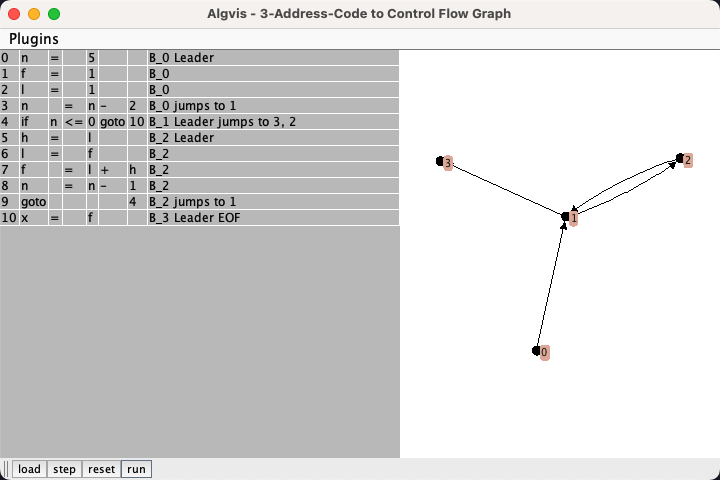
\includegraphics[width=0.8\textwidth]{fig/Screenshot_TacToCFG.png}
  \caption{Das "3-Address-Code zu Grundblöcken" Plugin}
  \label{fig:TACtoCFG}
\end{figure}

Das Plugin zur Generierung eines Kontrollflussgraphen aus 3-Address-Code 
ist eine Erweiterung des Plugins zur Erstellung von Grundblöcken.

Es erweitert das im letzten Abschnitt behandelte Programm indem es
neben der Tabelle einen Kontrollflussgraphen anzeigt.

Um dies zu realisieren, wurden neben einem Graphen, zwei Map-Objekte hinzugefügt. 
Eines in der Plugin-Klasse, um zu verfolgen, welche Grundblöcke bereits einen 
Knoten im Graphen besitzen und eines in der Algorithmus-Klasse, um festzuhalten,
welche Grundblöcke auf andere folgen.

Die Methode zum Zuordnen der Instruktionen zu ihren Grundblöcken (\cref{cde:mapBlocks})
wurde erweitert, sodass die Nachfolger der Grundblöcke nicht nur im Kommentar,
sondern auch in der Map erfasst werden:
\newpage
\begin{lstlisting}[language=Java, caption={Erweiterung der \textit{mapAddressesToItsBlock}-Methode}, label={cde:mapBlocks2}]
...
if(code.getLast().equals(instruction)) {
  if(instruction.canJump()){
    StringBuilder postfix = new StringBuilder(" jumps to ");
    ThreeAddressCodeInstruction nextInstruction = 
      instruction.nextPossibleInstructionAdresses().stream()
      .map(code::get)
      .min(ThreeAddressCodeInstruction::compareTo)
      .get();
    postfix.append(getSortedLeaders().indexOf(nextInstruction));
    successorMap.put(getPreviousLeader(address), new HashSet<>(Set.of(nextInstruction)));
    instruction.setComment(instruction.getComment() + postfix.toString());
  }
}else if(leaders.contains(code.get(address+1))) {
  StringBuilder postfix = new StringBuilder(" jumps to ");
  List<ThreeAddressCodeInstruction> nextInstructions = 
    instruction.nextPossibleInstructionAdresses().stream()
    .map(code::get)
    .toList();
  for (int i = 0; i < nextInstructions.size(); i++) {
    postfix.append(getSortedLeaders().indexOf(nextInstructions.get(i)));
    if(i+1<nextInstructions.size())
      postfix.append(", ");
  }
  successorMap.put(getPreviousLeader(address), new HashSet<>(nextInstructions));
  instruction.setComment(instruction.getComment() + postfix);
}

if(code.getLast().equals(instruction)) {
  instruction.setComment(instruction.getComment() + " EOF");
}
\end{lstlisting}
In den If Statements werden die Blöcke, in denen die Instruktionen die als nächstes
ausgeführt werden, ermittelt und an das Ende des Kommentars gehangen. Ausserdem
werden die Adressen der nächsten Instruktionen in die \textit{successorMap}
zugefügt
\footnote{Im Plugin \glqq 3-Address-Code to Basic Block\grqq\ existiert diese Map nicht, 
daher hat die Methode dort die beiden Befehle auch nicht.}.



\newpage
Die \textit{refreshGuiElements()}-Methode wurde auch um folgende Zeilen erweitert:
\begin{lstlisting}[language=Java, caption={Aktualisieren der Tabelle}, label={cde:refresh2}]
//set CFG
List<ThreeAddressCodeInstruction> leaders = 
  currentPluginInstance.getSortedLeaders();
for (ThreeAddressCodeInstruction leader : 
  currentPluginInstance.getSortedLeaders()) {
  //add new Nodes
  if(!nodeMap.containsKey(leader)) {
    Node node = new Node();
    nodeMap.put(leader, node);
    controlFlowGraph.addNode(nodeMap.get(leader));
  }
  controlFlowGraph.setLabelOfNode(
    nodeMap.get(leader), Integer.toString(leaders.indexOf(leader))
  );
}
//add all edges
Map<ThreeAddressCodeInstruction
  , Set<ThreeAddressCodeInstruction>> successorList = 
    currentPluginInstance.getSuccessorMap();
for (ThreeAddressCodeInstruction source:successorList.keySet()) {
  Node sourceNode = nodeMap.get(source);
  for (ThreeAddressCodeInstruction destination:
    successorList.get(source)) {
    Node destinationNode = nodeMap.get(destination);
    controlFlowGraph.addEdge(new Edge(sourceNode, destinationNode));
  }
}
\end{lstlisting}
In der ersten Schleife wird für jeden (bis zu diesem Schritt) 
gefundenen Leader ein Knoten im Graphen erstellt, wenn dieser 
noch nicht hinzugefügt worden ist. Das Label jedes Leaders aktualisiert,
da nicht zu jedem Zeitpunkt jeder Leader gefunden kann nicht davon ausgegangen werden,
dass die Label aus dem letzten Schritt noch aktuell sind.\\
In der zweiten Schleife werden für alle Leader Kanten zu den erkannten Nachfolgern gezeichnet.



\newpage
\subsection{Analyse von erreichenden Definitionen}
Das Plugin zur Visualisierung der Analyse der erreichenden Definitionen (\cref{fig:reachingDefinitions})
hat eine weitere Tabelle, in der Datenflusswerte angezeigt werden.
\begin{figure}[h]
  \centering
  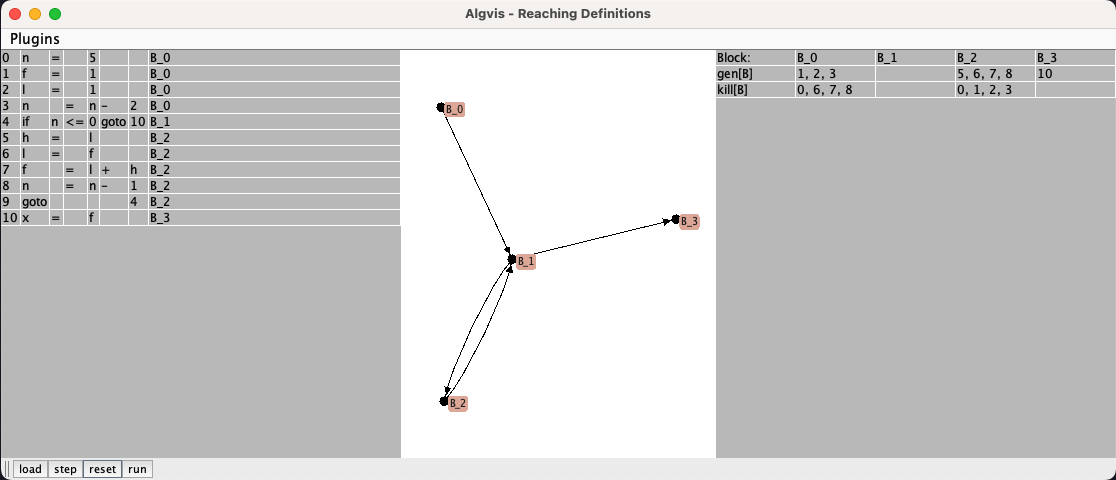
\includegraphics[width=0.99\textwidth]{fig/Screenshot_ReachingDefinitions.png}
  \caption{Das "Reaching Definitions" Plugin}
  \label{fig:reachingDefinitions}
\end{figure}

Da sich sowohl der Kontrollflussgraph, als auch der 3-Address-Code im
Verlaufe des Programmes nicht verändern, werden diese nicht in der
\textit{refreshGuiElements()}-Methode behandelt, sondern in der \textit{reset()}-Methode.
Da in dieser ein neues Objekt der Algorithmusklasse erstellt wird und
sich der Code nur dort ändern kann.

In der \textit{refreshGuiElements()}-Methode verändert sich dementsprechend
nur die Tabelle, in der Datenflusswerte angezeigt werden.

Diese berechnen wir, wie in \cref{t:rd} erläuftert, in der Algorithmusklasse:

Die $gen_B$ und $kill_B$-Mengen berechnen wir als Maps für jeden Grundblock $B$: 
\begin{lstlisting}[language=Java, caption={Berechnung einer $gen$ und $kill$-Menge}, label={cde:gen}]
//gen
Set<Integer> currentGenSet = gen.get(block);
for (int i = block.lastAddress(); i >= block.firstAddress(); i--) {
  ThreeAddressCodeInstruction currentInstruction = code.get(i);
  if(!currentInstruction.writesValue())
    continue;
  boolean newVar = true;
  for (int j : currentGenSet) {
    if(currentInstruction.getDestination().equals(code.get(j).getDestination()))
      newVar = false;
  }
  if(newVar)
    currentGenSet.add(i);
}
//kill
Set<Integer> currentKillSet = kill.get(block);
for (Integer i:currentGenSet) {
  for (int j = 0; j < code.size(); j++) {
    if(!code.get(j).writesValue())
      continue;
    if(j == i)
      continue;
    if(code.get(j).getDestination().equals(code.get(i).getDestination()))
      currentKillSet.add(j);
  }
}
\end{lstlisting}

Beim Durchlaufen des Algorithmus berechnen wir
in einem Schritt die $in[B]$ und $out[B]$ Mengen für einen Grundblock $B$.
Wenn diese sich von der in der letzten Iteration berechneten Menge
unterscheidet, ist unser Fixpunkt noch nicht erreicht.\\

Da wir nicht nur die aktuellen $in$ und $out$-Mengen darstellen wollen,
sondern alle, werden diese in einer Liste gespeichert.

Die $in_i[B]$-Menge wird als Vereinigung aller $out[B]$-Mengen der Vorgänger
des Blocks $B$ berechnet (\cref{cde:rdIn}):
\begin{lstlisting}[language=Java, caption={Berechnen der $in$-Menge}, label={cde:rdIn}]
Set<String> currentIn =  new HashSet<>();
for (BasicBlock ancestorBlock:ancestorBlocks) {
  Set<String> lastOut = (currentIteration>0) 
    ? out.get(currentIteration-1).get(ancestorBlock)
    : Set.of();//Leeres Set wenn es kein vorherige Iteration gibt
  currentIn.addAll(lastOut);
}
\end{lstlisting}

Die $gen_B$ und $kill_B$ Mengen wurden auf den Adressen der Instruktionen definiert,
werden jedoch als Adressen benötigt, daher werden sie wie folgt konvertiert:

\begin{lstlisting}[language=Java, caption={Konvertierung der $gen$-Menge}, label={cde:genConv}]
List<String> generatedIdentifiers = 
  gen.get(currentBlock).stream()
    .map(j -> code.get(j).getDestination())
    .toList();
List<String> killedIdentifiers = 
  kill.get(currentBlock).stream()
    .map(j -> code.get(j)
    .getDestination())
    .toList();
\end{lstlisting}

Um nun die $out[B]$-Menge zu berechen, werden alle Elemente der $kill_B$-Menge aus
einer Kopie der $in[B]$-Menge entfernt. Anschließend fügen wie alle Elemente der
$gen_B$-Menge hinzu:
\begin{lstlisting}[language=Java, caption={Berechnung der $out$-Menge}, label={cde:rdOut}]
Set<String> currentOut = new HashSet<>(currentIn);
currentOut.removeAll(killedIdentifiers);
currentOut.addAll(generatedIdentifiers);
\end{lstlisting}

Um die berechneten Datenflusswerte anzuzeigen, wird die Tabelle 
wie im Beispiel (\cref{tab:fib-rd}) befüllt:

Die erste Zeile dient als Überschriftszeile für die Grundblöcke.
Die zweite und dritte Zeile befüllen die $gen_B$ und $kill_B$ Mengen(\cref{cde:visgenkill}):
\begin{lstlisting}[language=Java, caption={Berechnung der $out$-Menge}, label={cde:visgenkill}]
dataFlow.setValueAt("gen[B]", 1, 0);
dataFlow.setValueAt("kill[B]", 2, 0);
for (int col = 0; col < basicBlocks.size(); col++) {
  BasicBlock block = basicBlocks.get(col);
  String genBlock = collectStringSet(
    pluginInstance.getGen().get(block).stream()
      .map(String::valueOf)
      .collect(Collectors.toSet())
    );
  String killBlock = collectStringSet(
    pluginInstance.getKill().get(block).stream()
      .map(String::valueOf)
      .collect(Collectors.toSet())
    );
  dataFlow.setValueAt(genBlock, 1, col+1);
  dataFlow.setValueAt(killBlock, 2, col+1);
}
\end{lstlisting}
Die Methode \textit{collectStringSet} ist hier eine Helfermethode, welche ein
Set an Strings zu einem String kombiniert, indem die einzelnen Elemente durch Kommas getrennt werden.

In den folgenden Zeilen werden die $in[B]$ und $out[B]$ Mengen aufgelistet.
Da in der letzten Iteration eventuell noch nicht alle Mengen bestimmt worden sind, 
wird für die unbestimmten Mengen ein Platzhalter-Set mit dem Element \glqq -\grqq  eingefügt:

\begin{lstlisting}[language=Java, caption={Visualisierung der $in$ und $out$-Mengen}, label={cde:visinout}]
for (int i = 0; i < inTable.size();i++) {
  int rowIndex = (i*2)+3;
  Map<BasicBlock, Set<String>> inMap = inTable.get(i);
  Map<BasicBlock, Set<String>> outMap = outTable.get(i);
  dataFlow.setValueAt("in[B]^"+i, rowIndex, 0);
  dataFlow.setValueAt("out[B]^"+i, rowIndex+1, 0);
  for (int j = 0; j < basicBlocks.size(); j++) {
    Set<String> inBlock = inMap.getOrDefault(basicBlocks.get(j), Set.of("-"));
    String inString = collectStringSet(inBlock);
    dataFlow.setValueAt(inString, rowIndex, j+1);

    Set<String> outBlock = outMap.getOrDefault(basicBlocks.get(j), Set.of("-"));
    String outString = collectStringSet(outBlock);
    dataFlow.setValueAt(outString, rowIndex+1, j+1);
  }
}
\end{lstlisting}

\newpage
\subsection{Analyse von lebendigen Variablen bezüglich Grundblöcken}
\begin{figure}[h]
  \centering
  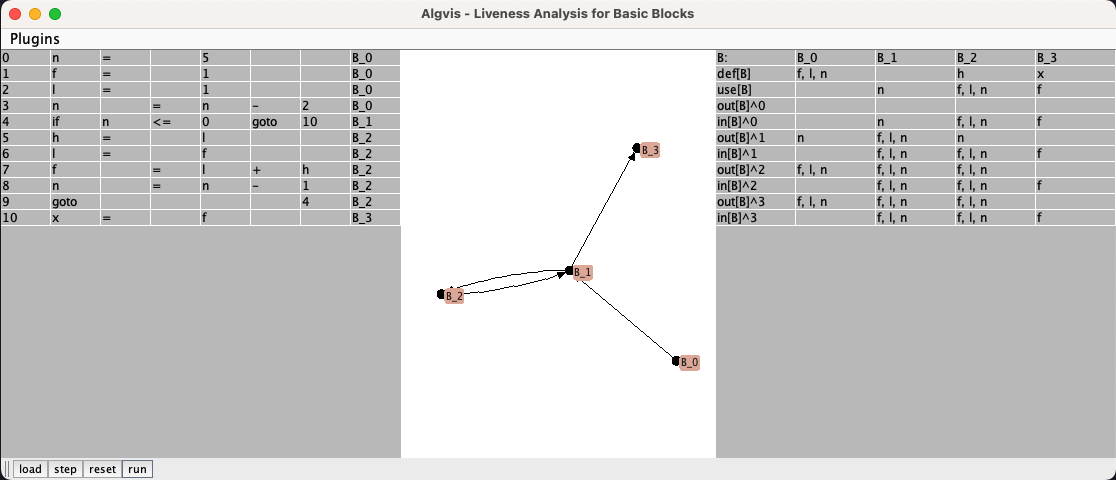
\includegraphics[width=0.99\textwidth]{fig/Screenshot_LivenessBb.png}
  \caption{Das "Liveness Analysis for Basic Blocks" Plugin}
  \label{fig:livenessAnalysisBB}
\end{figure}
Im folgenden Kapitel wird die Implementation des Algorithmus für die Liveness
Analysis besprochen. Da der Aufbau der Gui identisch zu dem Plugin für errichende
Definitionen ist, wird darauf nicht erneut eingegangen.

Da die Datenflussrichtung rückwärts läuft, wird die $out[B]$-Menge wie folgt
bestimmt:
\begin{lstlisting}[language=Java, caption={Berechnung der $out$-Menge}, label={cde:laIn}]
Set<String> currentOut = new HashSet<>();
for (BasicBlock successor:successorBlocks) {
  Set<String> lastInSuccessor = (currentIteration>0)
    ? in.get(currentIteration-1).get(successor)
    : Set.of();
  currentOut.addAll(lastInSuccessor);
}
\end{lstlisting}

\newpage
Um den Algorithmus wie in \cref{t:la} zu implementieren, müssen für alle
Grundblöcke $B$ die $def_B$ und $use_B$ Mengen definiert werden.
Dies geschieht wie folgt (\cref{cde:laDefUse}):
\begin{lstlisting}[language=Java, caption={Berechnung der $def$ und $use$-Mengen}, label={cde:laDefUse}]
//def
Set<String> currentDefSet = def.get(block);
for (int i = block.lastAddress(); i >= block.firstAddress(); i--) {
  ThreeAddressCodeInstruction instruction = code.get(i);
  if(!instruction.writesValue())
    continue;
  String identifier = instruction.getDestination();
  currentDefSet.add(identifier);
  for (int j = 0; j < i; j++) {
    if(code.get(j).getUsedIdentifiers().contains(identifier))
      currentDefSet.remove(identifier);
  }
}
//use
Set<String> currentUseSet = use.get(block);
for (int i = block.lastAddress(); i >= block.firstAddress(); i--) {
  ThreeAddressCodeInstruction instruction = code.get(i);
  for (String used:instruction.getUsedIdentifiers()) {
    currentUseSet.add(used);
    for (int j = block.firstAddress(); j < i; j++) {
      if(code.get(j).writesValue() && code.get(j).getDestination().equals(used))
        currentUseSet.remove(used);
    }
  }
}
\end{lstlisting}
Und die Transferfunktion wird wie folgt berechnet:

\begin{lstlisting}[language=Java, caption={Berechnung der $out$-Menge}, label={cde:laOut}]
Set<String> currentIn = new HashSet<>(currentOut);
currentIn.removeAll(def.get(currentBlock));
currentIn.addAll(use.get(currentBlock));
\end{lstlisting}

\newpage
\subsection{Analyse von lebendigen Variablen bezüglich einzelnen Instruktionen}
\begin{figure}[h]
  \centering
  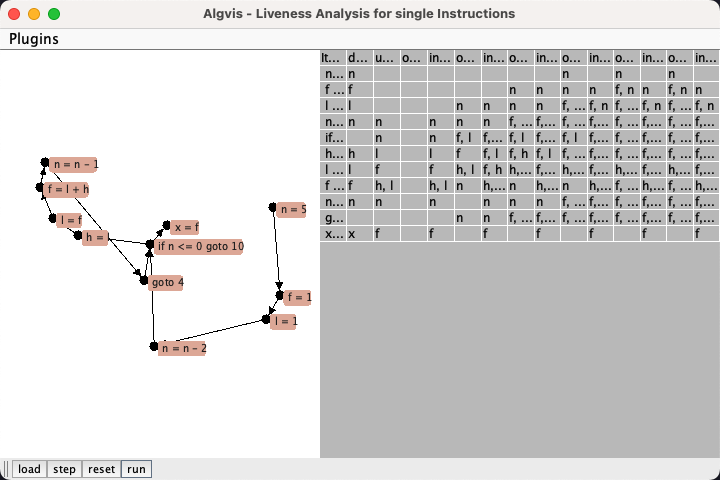
\includegraphics[width=0.8\textwidth]{fig/Screenshot_LivenesTAC.png}
  \caption{Das "Liveness Analysis for Three Address Code" Plugin}
  \label{fig:livenessAnalysisTAC}
\end{figure}
Durch die im letzten Abschnitt definierte Liveness Analyse lässt sich mit wenigen
Iterationen eine konservative Abschätzung der benötigten Register machen.
Da sich jedoch auch innerhalb eines Grundblocks die Werte der Liveness Analyse ändern können,
kann die liveness Analyse auch auf einzelnen Instruktionen geführt werden, 
hierbei werden jedoch wesentlich mehr Iterationen benötigt, bis der Fixpunkt erreicht ist.\\

Dieses Plugin (\cref{fig:livenessAnalysisTAC}) implementiert eben diese Analyse. Indem es alle Instruktionen
in einem Graphen anzeigt und deren Datenflusswerte in einer Tabelle.

Die Transferfunktion bleibt identisch zur liveness Analyse auf Grundblöcken.
Jedoch müssen die $use_i$ und $def_i$-Mengen auf einzelnen Instruktionen $i$
definiert werden:
\begin{itemize}
  \item Die $use_i$-Menge umfasst trivialer Weise alle Adressen die in ihrer Instruktion $i$
    benötigt werden.
  \item Die $def_i$-Menge ist definiert durch: 
    Alle Instruktionen, die einen Wert definieren haben ein Element in ihrer
    $def_i$ Menge, nämlich die Adresse in der dieser Wert gespeichert wird.
    Wenn eine Instruktion keinen Wert speichert, gilt $def_i=\emptyset$.
\end{itemize}

\newpage
%! TeX root: thesis.tex
\section{Verwandte Arbeiten}

Wie im \cref{motiv} bereits erwähnt, gibt es einige andere Arbeiten,
welche ähnliche Aufgaben haben:\\

Eine davon ist die STUPSToolbox\cite{toolbox} programmiert von Fabian Ruhland
\footnote{Warum kommt mir der Name so bekannt vor? :)}
und erweitert von Isabel Wingen.\\
Diese Toolbox enthält einige Funktionaliäten für die Arbeit mit Automaten
und Grammatiken. Ursprünglich war die Idee, diese Toolbox weiter zu entwickeln,
jedoch funktioniert diese leider mittlerweile nicht mehr ohne weiteres. Daher wurde
sich dagegen entschieden, diese Toolbox zu erweitern oder instand zu setzen.\\

Ein Tool, mit dem auch liveness Analyse gemacht werden kann ist der
Data Flow Analysis Visualizer\cite{dfav}. Dies ist eine Abschlussarbeit\cite{dfavpres}
eines Compilerdesign Kurses der UCSD
\footnote{University of California San Diego}.
Leider kann in diesem Programm nur JavaScript-Code eingegeben werden
und auch nur eine Liveness Analyse auf einzelnen Instruktionen ausgeführt werden.

Letztlich gibt es noch ein Tool namens VisOpt\cite{VisOpt}.
In diesem kann man Jova\footnote{Eine Subsprache von Java}-Code eingeben,
ihn in 3-Address-Code übersetzen lassen und sich eine Vielzahl 
von Optimierungsmöglichkeiten visualisieren lassen.\\
Leider ist es jedoch nicht möglich, direkt 3-Address-Code einzugeben,
sich Grundblöcke anzeigen zu lassen oder eine reaching Definitions Analyse
durchzuführen.\\

\newpage
\section{Ausblick}
Das in dieser Arbeit entwickelte Framework bietet ein Fundament, 
um viele Analyse- und Optimierungsalgorithmen zu visualisieren.\\
Leider ist es im vorgegebenen Zeitrahmen nicht möglich gewesen, mehr als
die in der Arbeit besprochenen Plugins zu schreiben.\\

Folgende Algorithmen können ohne Erweiterung des Frameworks implementiert werden:
\begin{itemize}
  \item Konstantenpropagation
  \item Verfügbare Ausdrücke
  \item Eliminierung von Redundanz
\end{itemize}

Durch Implementierung von Automaten im Framework können außerdem weitere 
Konzepte visualisiert werden, die Studenten des Compilerbaus helfen könnten:
\begin{itemize}
  \item Erstellen von Lexern für die Tokenisierung
    \begin{enumerate}
      \item nicht-determinischer endlicher Automat (NEA)
      \item deterministischer endlicher Automat (DEA)
      \item minimierter DEA
    \end{enumerate}
    Ausserdem auch Durchführung einer Tokenisierung von Quellcode
  \item Erstellen von Parsern für den Bau von Syntaxbäumen
    \begin{enumerate}
      \item Top-Down parsing
      \item Bottom-Up parsing
    \end{enumerate}
  \item Generierung von 3-Address-Code aus einem Syntaxbaum
\end{itemize}



\newpage
\section{Herausforderungen und Fazit}
Das im Exposé vereinbarte Ziel dieser Bachelorarbeit war es, folgende Konzepte zu visualisieren:
\begin{itemize}
  \item Das Bauen eines Kontrollflussgraphen aus 3-Addres-Code
  \item Das Visualisieren von Constant Folding
  \item Das Visualisieren von liveness Analysen
  \item Und das Visualisieren von reaching Definitions
\end{itemize}

Leider war es aufgrund von falsch eingeschätztem Arbeitsaufwand nicht möglich, 
den constant Folding Algorithmus zu implementieren.\\

Das Implementieren des Frameworks war hingegen sehr erfolgreich.\\
Es war möglich ein minimales Interface zu erstellen, welches alle
Funktionen des Frameworks abbilden kann. Mit diesem können neue Plugins
mit sehr geringem Aufwand hinzugefügt werden.\\

Ausserdem wurde das Framework samt Plugins einer Gruppe 
Student*innen des Compilerbau Moduls vorgestellt.
Das Feedback der Studierenden war positiv, die vorgestellten Plugins
seien nützlich, um zum Beispiel Übungsaufgaben zu bearbeiten,
da die Lösung Schritt für Schritt abgleichbar ist.\\



% \appendix
% %!TeX root: thesis.tex
\section{Codebeispiele}
\begin{lstlisting}[language=Java, caption={Generieren der ID für eine Kante}, label={cde:edge-id}]
public String getID(){
  return "("+sourceNode.getId()+") -> ("+targetNode.getId()+")";
}
\end{lstlisting}

\begin{lstlisting}[language=Java, caption={Konstruktor der Klasse ThreeAddressCodeInstruction}, label={cde:graph-constructor}]
public Graph(Location location){
  this.location = location;
  exportedPanel = new JPanel(new BorderLayout());
  switch(location){...} // Groesse des exportierten JPanels festlegen
  
  nodes = new HashSet<>();
  edges = new HashSet<>();
  
  graph = new MultiGraph("Graph");
  graph.setAttribute("ui.stylesheet", ...); // stylesheet festlegen
  viewer = new SwingViewer(graph, ...); // threading festlegen
  View view = viewer.addDefaultView(false);

  layout = new LinLog();
  viewer.enableAutoLayout(layout);

  exportedPanel.add((Component) view, BorderLayout.CENTER);
}
\end{lstlisting}
\begin{lstlisting}[language=Java, caption={Implementierung der addNode(Node) Methode}, label={cde:graph-addNode}]
  public void addNode(Node newNode){
    if(nodes.contains(newNode))
      return;
    nodes.add(newNode);
    graph.addNode(newNode.getId());
    layout.shake();
  }
\end{lstlisting}
\begin{lstlisting}[language=Java, caption={Implementierung der setLabelOfNode(Node, String) Methode}, label={cde:graph-labelNode}]
  public void setLabelOfNode(Node Node, String label){
    if(nodes.contains(newNode))
      graph.getNode(node).setAttribute("ui.label", label);
  }
\end{lstlisting}

\begin{lstlisting}[language=Java, caption={Implementierung der setValueAtMethode(Object, int, int) Methode}, label={cde:setValueAt}]
  public void setValueAt(Object value, int rowIndex, int colIndex){
    if(value == null)
      value = "";
    try{
      data[rowIndex][colIndex] = value.toString();
      TableModelEvent event = new TableModelEvent(...);
      listeners.forEach(l->l.tableChanged(event));
    }catch(ArrayIndexException e){
      // Error handling
    }
  }
\end{lstlisting}


\begin{lstlisting}[language=Java, caption={Implementierung der resizeTable(int, int) Methode}, label={cde:resizeTable}]
public void resizeTable(int rows, int cols) {
  if(rows==tableModel.getRowCount() 
  && cols == tableModel.getColumnCount())
    return;
  tableModel = new DataTableModel(rows, cols);
  this.setModel(tableModel);
}
\end{lstlisting}

\begin{lstlisting}[language=Java, caption={Implementierung der highlightLine(int) Methode}, label={cde:highlightLine}]
public void highlightLine(int line) {
  this.clearSelection();
  if (line == 0)
    return;
  try {
    this.addRowSelectionInterval(line, line);
  }catch (IllegalArgumentException e){
    ... //Handle wrong lines error
  }
    }
}
\end{lstlisting}

\begin{lstlisting}[language=Java, caption={Implementierung der getToolTipText(MouseEvent) Methode}, label={cde:tooltip}]
  public String getToolTipText(MouseEvent mouseEvent) {
    String tip = null;
    Point p = mouseEvent.getPoint();

    int rowIndex = rowAtPoint(p);
    int colIndex = columnAtPoint(p);

    try{
      if(rowIndex<getRowCount() && rowIndex> -1
      && colIndex<getColumnCount() && colIndex> -1)
        tip = tableModel.getValueAt(rowIndex, colIndex).toString();
    }catch (NullPointerException ignored){}
    
    return tip;
  }
\end{lstlisting}

\begin{lstlisting}[language=java, caption={Implementierung der resizeColumnDisplay() Methode}, label={cde:resize}]
  public void resizeColumnDisplay() {
    TableColumnModel columnModel = this.getColumnModel();
    for (int i = 0; i < columnModel.getColumnCount()-1; i++) {
      int width = 0;
      for (int j = 0; j < tableModel.getRowCount(); j++) {
        TableCellRenderer renderer = this.getCellRenderer(j, i);
        Component component = this.prepareRenderer(renderer, j, i);
        width = Math.max(component.getPreferredSize().width+2, width);
      }
      columnModel.getColumn(i).setMinWidth(width);
      columnModel.getColumn(i).setMaxWidth(width);
    }
    int width = 10;
    for (int j = 0; j < tableModel.getRowCount(); j++) {
      TableCellRenderer renderer = this.getCellRenderer(j, columnModel.getColumnCount()-1);
      Component component = this.prepareRenderer(renderer, j, columnModel.getColumnCount()-1);
      width = Math.max(component.getPreferredSize().width+2, width);
    }
    columnModel.getColumn(columnModel.getColumnCount()-1).setMinWidth(width);
    columnModel.getColumn(columnModel.getColumnCount()-1).setMaxWidth(this.getMaximumSize().width);
  }
\end{lstlisting}




\begin{lstlisting}[language=java, caption={Konstruktor der Klasse ThreeAddressCodeInstruction}, label={cde:taci-constructor}]
public ThreeAddressCodeInstruction(String rawInput, int address){
  ...
  String[] pieces = rawInput.split(" ");
  switch (pieces.length) {
    case 2 -> ... //Unbedingter Sprung goto X
    case 3 -> ... //Kopierbefehl X = Y
    case 4 -> { //entweder unaere Operation oder ein bedingter Sprung
      switch(pieces[2]){
        case "-" -> ... //Unaere Operation X = - Y
        case "goto" -> {//ein bedingter Sprung
          switch(pieces[0]){
            case "if" -> ... //bedingter Sprung if Y goto X
            case "ifFalse" -> ... //bedingter Sprung ifFalse Y goto X
          }
        }
      }
    case 5 -> ... //Binaere Operation X = Y op Z
    case 6 -> { //bedingter Sprung
      switch(pieces[2]){
        case "<" -> ...//if Y < Z goto X
        case ">" -> ...//if Y > Z goto X
        case "<=" -> ...//if Y <= Z goto X
        case ">=" -> ...//if Y >= Z goto X
        case "==" -> ...//if Y == Z goto X
        case "!=" -> ...//if Y != Z goto X
      }
    }
    ...
 }
\end{lstlisting}

\begin{lstlisting}[language=Java, caption={Der Konstruktor der ThreeAddressCode Klasse}, label={cde:tac-constructor}]
public ThreeAddressCode(String raw){
  List<String> inputLines = raw.lines().toList();
  code = new ArrayList<>(inputLines.size());
  for (int i = 0; i < inputLines.size(); i++) {
    code.add(new ThreeAddressCodeInstruction(inputLines.get(i), i));
  }
  basicBlocks = toBBList(code);
}
\end{lstlisting}

\begin{lstlisting}[language=Java, caption={Zusammenfassung der toBBList() Methode}, label={cde:bb-gen}]
private static List<BasicBlock> toBBList(List<...> code){
  Set<ThreeAddressCodeInstruction> leaders = new HashSet<>(1);
  if(!code.isEmpty()) //die erste Instruktion ist immer Leader
    leaders.add(code.get(0));
  for (int i = 0; i < code.size(); i++) {
    ... // Finde alle Leader 
  }
  List<ThreeAddressCodeInstruction> sortedLeaders = leaders.stream().sorted(Comparator.comparingInt(ThreeAddressCodeInstruction::getAddress)).toList();
  
  // Finde die letzte Instruktion jedes Grundblockes
  List<Integer> firstAddresses = sortedLeaders.stream()
                .map(ThreeAddressCodeInstruction::getAddress)
                .toList();
  List<Integer> lastAddresses = new ArrayList<>(leaders.size());
  for (int i = 1; i < sortedLeaders.size(); i++) {
    lastAddresses.add(firstAddresses.get(i)-1);
  }
  lastAddresses.add(code.getLast().getAddress());
  
  List<List<Integer>> fAOS = new ArrayList<>(leaders.size());
  for (int lastAddress : lastAddresses) {
    ... // Bestimme die Addressen der Nachfolger
  }
 

  // Setze die Listen zu einer BasicBlock Liste zusammen
  List<BasicBlock> basicBlocks= new ArrayList<>(leaders.size());
  for (int i = 0; i < firstAddresses.size(); i++) {
    int firstAddress = firstAddresses.get(i);
    int lastAddress = lastAddresses.get(i);
    List<Integer> successors = fAOS.get(i);
    BasicBlock basicBlock = new BasicBlock(
      firstAddress, lastAddress, successors
    );
    basicBlocks.add(basicBlock);
  }
  return basicBlocks;
}
\end{lstlisting}
\newpage

\begin{lstlisting}[language=Java, caption={Ausschnitt der toBBList()-Methode zum finden aller Leader}, label={cde:bb-leader}]
for (int i = 0; i < code.size(); i++) {
  if(code.get(i).canJump()){
    ThreeAddressCodeInstruction destination = code.get(
      Integer.parseInt(code.get(i).getDestination())
    );
    leaders.add(destination);
    if(i+1<code.size()) 
      leaders.add(code.get(i+1));
} }
\end{lstlisting}

\begin{lstlisting}[language=Java, caption={Zusammenfassung der toBBList() Methode}, label={cde:bb-successor}]
List<List<Integer>> fAOS = new ArrayList<>(leaders.size());
for (int lastAddress : lastAddresses) {
  List<Integer> successors = new ArrayList<>(0);
  fAOS.add(successors);
  switch (code.get(lastAddress).getOperation()) {
    case jmp -> 
      successors.add(
        Integer.valueOf(code.get(lastAddress).getDestination())
      );
    case booleanJump, negatedBooleanJump, 
         eqJump, geJump, gtJump, leJump, ltJump, neJump -> {
      successors.add(
        Integer.valueOf(code.get(lastAddress).getDestination())
      );
      if (lastAddress+1 < code.size())
        successors.add(lastAddress + 1);
    }
    default -> {
      if (lastAddress+1 < code.size())
        successors.add(lastAddress + 1);
} } }
\end{lstlisting}
\begin{lstlisting}[language=Java, caption={Bestimmmen der gen Menge für erreichende Definitionen}, label={cde:rd_gen}]
for(BasicBlock block:basicBlocks){
  Set<Integer> currentGenSet = gen.get(block);
  for (int i = block.lastAddress(); i >= block.firstAddress(); i--) {
    ThreeAddressCodeInstruction currentInstruction = code.get(i);
    if(!currentInstruction.writesValue())
      continue;
    boolean newVar = true;
    for (int j : currentGenSet) {
      if(currentInstruction.getDestination().equals(code.get(j).getDestination()))
        newVar = false;
    }
    if(newVar)
      currentGenSet.add(i); 
  }
}
\end{lstlisting}

\begin{lstlisting}[language=Java, caption={Bestimmmen der kill Menge für erreichende Definitionen}, label={cde:rd_kill}]
for(BasicBlock block:basicBlocks){
  Set<Integer> currentKillSet = kill.get(block);
  for (Integer i:currentGenSet) {
    for (int j = 0; j < code.size(); j++) {
      if(!code.get(j).writesValue())
        continue;
      if(j == i)
        continue;
      if(code.get(j).getDestination().equals(code.get(i).getDestination()))
        currentKillSet.add(j);
    }
  }
}
\end{lstlisting}

\begin{lstlisting}[language=Java, caption={Bestimmmen der Menge der Vorfahren für erreichende Definitionen}, label={cde:rd_anc}]
for (BasicBlock block:basicBlocks) {
  List<Integer> firstAddressesOfSuccessors = block.firstAddressesOfSuccessors();
  for (int address:firstAddressesOfSuccessors) {
    for (BasicBlock potentialSuccessor:basicBlocks) {
      if(potentialSuccessor.firstAddress() == address)
        ancestors.get(potentialSuccessor).add(block);
    }
  }
}
\end{lstlisting}


%%%%%%%%%%%%%%%%%%%%%%%%%%%%%%%%%%%%%%%%%%%%%%%%%%%%%%%%%%%%%%%%%%%%%%%%%%%%%%%%
%% (Ende) Der Inhalt der Arbeit                                               %%
%%%%%%%%%%%%%%%%%%%%%%%%%%%%%%%%%%%%%%%%%%%%%%%%%%%%%%%%%%%%%%%%%%%%%%%%%%%%%%%%

\backmatter
\listoffigures
\listoftables

\clearpage
\bibliography{references}
%% Depending on Language, use german alphadin or original alpha
\iflanguage{ngerman}{
  \bibliographystyle{alphadin}
}{
  \bibliographystyle{alpha}
}

\end{document}
